% \documentclass{article}
\documentclass[letterpaper,USenglish]{lipics-v2016}
%This is a template for producing LIPIcs articles. 
%See lipics-manual.pdf for further information.
%for A4 paper format use option "a4paper", for US-letter use option "letterpaper"
%for british hyphenation rules use option "UKenglish", for american hyphenation rules use option "USenglish"
% for section-numbered lemmas etc., use "numberwithinsect"
\def\OPTIONConf{0}%
\def\OPTIONArxiv{0}%
 
\usepackage{microtype}%if unwanted, comment out or use option "draft"

%\graphicspath{{./graphics/}}%helpful if your graphic files are in another directory

\bibliographystyle{plainurl}% the recommended bibstyle

% Author macros::begin %%%%%%%%%%%%%%%%%%%%%%%%%%%%%%%%%%%%%%%%%%%%%%%%
\title{Toward Semantic Foundations for Interactive Programming Environments
%\footnote{This work was partially supported by someone.}
}
\titlerunning{Toward Semantic Foundations for Interactive Programming Environments} %optional, in case that the title is too long; the running title should fit into the top page column

%% Please provide for each author the \author and \affil macro, even when authors have the same affiliation, i.e. for each author there needs to be the  \author and \affil macros
\author[1]{Cyrus Omar}
\author[2]{Ian Voysey}
\author[3]{Michael Hilton}
\author[4]{Joshua Sunshine}
\author[5]{Claire Le Goues}
\author[6]{Jonathan Aldrich}
\author[7]{Matthew Hammer}
\affil[1]{Carnegie Mellon University, Pittsburgh, PA, USA\\
  \texttt{comar@cs.cmu.edu}}
\affil[2]{Carnegie Mellon University, Pittsburgh, PA, USA\\
  \texttt{iev@cs.cmu.edu}}
\affil[3]{Oregon State University, Corvallis, OR, USA\\
  \texttt{hiltonm@eecs.oregonstate.edu}}
\affil[4]{Carnegie Mellon University, Pittsburgh, PA, USA\\
  \texttt{sunshine@cs.cmu.edu}}
\affil[5]{Carnegie Mellon University, Pittsburgh, PA, USA\\
  \texttt{clegoues@cs.cmu.edu}}
\affil[6]{Carnegie Mellon University, Pittsburgh, PA, USA\\
  \texttt{aldrich@cs.cmu.edu}}
\affil[7]{University of Colorado Boulder, Boulder, CO, USA\\
  \texttt{matthew.hammer@colorado.edu}}

\authorrunning{C. Omar, I. Voysey, M. Hilton, J. Sunshine, C. Le Goues, J. Aldrich, and M. Hammer} %mandatory. First: Use abbreviated first/middle names. Second (only in severe cases): Use first author plus 'et. al.'

\Copyright{the authors}%mandatory, please use full first names. LIPIcs license is "CC-BY";  http://creativecommons.org/licenses/by/3.0/

% \subjclass{Dummy classification -- please refer to \url{http://www.acm.org/about/class/ccs98-html}}% mandatory: Please choose ACM 1998 classifications from http://www.acm.org/about/class/ccs98-html . E.g., cite as "F.1.1 Models of Computation". 
% \keywords{Dummy keyword -- please provide 1--5 keywords}% mandatory: Please provide 1-5 keywords
% Author macros::end %%%%%%%%%%%%%%%%%%%%%%%%%%%%%%%%%%%%%%%%%%%%%%%%%

%Editor-only macros:: begin (do not touch as author)%%%%%%%%%%%%%%%%%%%%%%%%%%%%%%%%%%
\EventEditors{John Q. Open and Joan R. Access}
\EventNoEds{2}
\EventLongTitle{Summit oN Advances in Programming Languages (SNAPL 2017)}
\EventShortTitle{SNAPL 2017}
\EventAcronym{SNAPL}
\EventYear{2017}
\EventDate{May 7--10, 2017}
\EventLocation{Asilomar, California}
\EventLogo{}
\SeriesVolume{42}
\ArticleNo{23}
% Editor-only macros::end %%%%%%%%%%%%%%%%%%%%%%%%%%%%%%%%%%%%%%%%%%%%%%%

\usepackage{etoolbox}
\usepackage{hyperref}

% \usepackage{srcltx}
% \usepackage{goodcharter}
% \usepackage{euler}

% \usepackage{joshuadunfield}
\usepackage{llproof}
%\usepackage{jdproof}
\usepackage{rulelinks}
\usepackage{listings}
\usepackage{graphicx}
\usepackage{wrapfig}
\usepackage{lmodern}
\usepackage{anyfontsize}
\usepackage{stmaryrd}
\SetSymbolFont{stmry}{bold}{U}{stmry}{m}{n}
\usepackage{amsmath,amsthm,amssymb}
\usepackage{thmtools,thm-restate}

\usepackage{enumerate}

% \usepackage[authoryear]{natbib}
% \bibpunct{(}{)}{;}{a}{}{,}

%\mprset{sep=1em}
\def\MathparLineskip{\lineskiplimit=0.9em\lineskip=0.8em plus 0.2em}

\declaretheoremstyle[
  bodyfont=\sl
]{mytheoremstyle}

\lstset{tabsize=2, 
basicstyle=\ttfamily, 
% keywordstyle=\sffamily,
commentstyle=\itshape\ttfamily\color{gray}, 
stringstyle=\ttfamily\color{red},
mathescape=false,escapechar=\#,
numbers=left, numberstyle=\scriptsize\color{gray}\ttfamily, language=ML, moredelim=[il][\sffamily]{?},showspaces=false,showstringspaces=false,xleftmargin=15pt, 
classoffset=0,belowskip=\smallskipamount, aboveskip=\smallskipamount
}
\lstloadlanguages{Java,VBScript,XML,HTML,ML}
\let\li\lstinline

\newcommand{\Hazel}[0]{\textsf{Hazel}}
\newcommand{\HazelEnv}[0]{\Hazel}

\newcommand{\RuleHead}[1]{\text{\raisebox{1em}[0pt]{\ensuremath{\mathsz{\ifnum\OPTIONConf=1 14pt\else 18pt \fi}{#1}}}}~~~~~}

\newcommand{\abort}{\keyword{abort}\xspace}
\newcommand{\xerrs}{\keyword{error}}
\newcommand{\errs}{\;\xerrs}
% \newcommand{\xmatchfailure}{\keyword{match-failure}}
% \newcommand{\matchfailure}{\;\xmatchfailure}
\newcommand{\inj}[1]{\keyword{inj}_{#1}\,}
\newcommand{\Inj}[1]{\inj{#1}}

\newcommand{\rulename}[1]{\text{\normalfont\textsf{#1}}}

\newcommand{\srctyperulename}[1]{\rulename{\textcolor{dDkRed}{S#1}}}
\newcommand{\srcintrorulename}[1]{\srctyperulename{{#1}Intro}}
\newcommand{\srcelimrulename}[1]{\srctyperulename{{#1}Elim}}

\newrulecommand{TAbort}{\targettyperulename{Abort}}

% \newcommand{\subrulename}[1]{\rulename{$\subtype${#1}}}
% \newrulecommand{SubInjDynsum}{\subrulename{Inj$+?$}}
% \newrulecommand{SubDynsumSum}{\subrulename{${+?}{+}$}}
% \newrulecommand{SubRefl}{\subrulename{Refl}}
% \newrulecommand{SubTrans}{\subrulename{Trans}}
% \newrulecommandONE{SubDynsumInj}{\subrulename{${+?}\Inj{#1}$}}

\newcommand{\tytrans}[1]{{|}{#1}{|}}
\newcommand{\ctxtrans}[1]{\tytrans{#1}}

\newcommand{\Rule}[2]{\textsf{#2}}

% \newtheorem{theorem}{Theorem}
\definecolor{Green}{rgb}{0.0, 0.99, 0.0}
\definecolor{light-gray}{rgb}{0.95, 0.95, 0.95}

\begin{document}
\maketitle

\begin{abstract}
% 
Programming language definitions assign formal meaning to {complete}
programs.
%
Programmers, however, spend a substantial amount of time interacting
with \emph{incomplete} programs -- programs with holes, type inconsistencies, binding inconsistencies and other problems -- using tools like program editors and
live programming environments (which interleave editing and
evaluation.)
%
Semanticists have paid comparatively little attention to incomplete programs and the 
interactions that programmers have with them. Consequently, the designers of these interactive programming tools lack foundational
semantic principles comparable to those available to language
designers. % Instead, they have had to rely on various \emph{ad hoc} heuristics. 
%
This paper serves as a vision statement for the HazelGrove project, which seeks to develop these ``missing'' semantic 
principles, starting from the first principles of type theory, and to apply these principles in the design of \HazelEnv, a new \emph{live lab notebook} programming
environment. 

% We propose:
% %
% a \textbf{static semantics for incomplete programs} that assigns static meaning to programs with \emph{holes}, \emph{type inconsistencies}, \emph{binding inconsistencies} and other local, transient problems; 
% %
% a \textbf{dynamic semantics for incomplete programs} that assigns dynamic meaning to incomplete programs and supports ``edit-and-resume'' functionality, thereby tightening the live programming feedback loop;  
% %
% an \textbf{action semantics} that captures the process of editing a program using structured edit actions and maintains a powerful semantic invariant: that every intermediate edit state can be assigned static and dynamic meaning according to the aforementioned semantics for incomplete programs; and 
% %
% a \textbf{statistical action suggestion semantics}, which serves as a foundation for advanced editor features, like semantic code completion and automatic program repair, that need to generate both \emph{semantically valid} and \emph{statistically likely} code snippets and actions.

% To ensure that these individual developments lead toward a coherent
% and practical \emph{theory of interactive programming}, we plan to
% integrate them into a \emph{live lab notebook} programming
% environment, \HazelEnv. By embracing a clean-slate integrative
% approach, we can investigate the semantics of novel constructs that
% are defined within programs but control the programming environment,
% notably \textbf{programmable edit action macros},
% \textbf{type-specific projection macros} and \textbf{semantic,
%   interactive documentation}.

% Although our proposed contributions are primarily {mathematical}, we
% will also conduct small \textbf{pilot studies} involving in order to
% 1) gather data for the action suggestion system; 2) iterate on
% \HazelEnv's design and evaluate whether our ``semantics-first'' tool
% design methodology can scale to produce a tool that allows programmers
% to productively engage in non-trivial (if not yet large-scale)
% programming tasks; and 3) evaluate whether the interactive
% documentation system we have proposed improves tutorial comprehension,
% relative to an approach that relies on non-interactive documentation.

\end{abstract}


\section{Introduction}

% Our research aims to bridge two historically distinct traditions: (1) the formal
% tradition, which has produced seminal advances by viewing programming languages,
% and therefore programs, as mathematical structures~(see e.g. \cite{pfpl,Pierce:2002hj}); and (2) the interaction design
% tradition, which has produced a number of innovative interactive programming
% tools by viewing programming as an interaction between a human programmer and a tool. We borrow from both traditions to propose 

% This paper envisions \Hazel, a clean-slate interactive programming
% environment equipped with a formal semantics that assigns meaning 
% to ``edit-time'' structures and interactions that have largely been 
% considered beyond the scope of the formal tradition to date. Figure~\ref{fig:hazel-mockup} shows a mockup of \HazelEnv's user interface,
% which we will reference throughout our discussion.

%\HazelEnv, like many existing 
Language-aware program editors (e.g. Eclipse
or Emacs, with the appropriate  
extensions installed \cite{gamma2004contributing}) provide a number of useful editor services, including (1)
syntax highlighting, (2)
the ability to inspect the type of an expression, (3)
the ability to jump to the binding site of a variable, and (4)
the ability to rename a variable in a semantics-preserving manner. 

When these editor services encounter \emph{complete programs} -- programs that are well-formed and semantically meaningful, according to the language definition -- they can rely on a variety of accompanying reasoning principles and program manipulation techniques. For example, a syntax highlighter for well-formed programs can be generated automatically 
from a context-free grammar \cite{DBLP:conf/tools/KrahnRV08,DBLP:conf/cc/BrandDHJJKKMOSVVV01} and the remaining editor services enumerated above can be realized 
by following the language's type and binding structure, as specified by a standard formal
semantics.

The problem, of course, is that many of the {edit states} encountered by a program editor do not correspond to complete programs. In these situations, many program editors simply disable various editor services. More advanced editors have developed various \emph{ad hoc}, poorly understood heuristics that attempt to recover from the problem and continue on.

\paragraph{Problem 1: Syntactically Malformed Edit States.} 
Textual program editors frequently encounter edit states
that are not well-formed with respect to the textual syntax of complete
programs. For example, consider a programmer in the midst of
constructing a call to a function \lstinline{std}: 
\[
\texttt{std(y, }
\]
There is a syntax
error at this moment in the editing process, so editor services that require a syntactically
complete program must be disabled. This is unsatisfying. Sophisticated editors like Eclipse, and editor generators like Spoofax \cite{DBLP:conf/oopsla/KatsV10}, use \emph{error recovery} heuristics that can support the continued provision 
of various services in some formally malformed states, by using secondary notational conventions (e.g. whitespace) to segregate malformed portions of the program  \cite{DBLP:conf/oopsla/KatsJNV09,DBLP:conf/sle/JongeNKV09}. These heuristics work most, but not all, of the time.

The alternative approach that we take for \HazelEnv is to build a
\emph{structure editor} -- a program editor where every edit state
maps onto a syntax tree, with \emph{holes} representing leaves of the tree
that have not yet been constructed.  This representation choice sidesteps the
problem of syntactically malformed edit states. Notice that in
Figure~\ref{fig:hazel-mockup}, the program fragment in cell
\textbf{(a)} contains holes, appearing as squares. This design also permits
non-textual \emph{projections} of expression, e.g. 
the 2D projection of a matrix value in cell \textbf{(b)}.
We will return to the topic of structure editors and projections below.


\begin{figure}
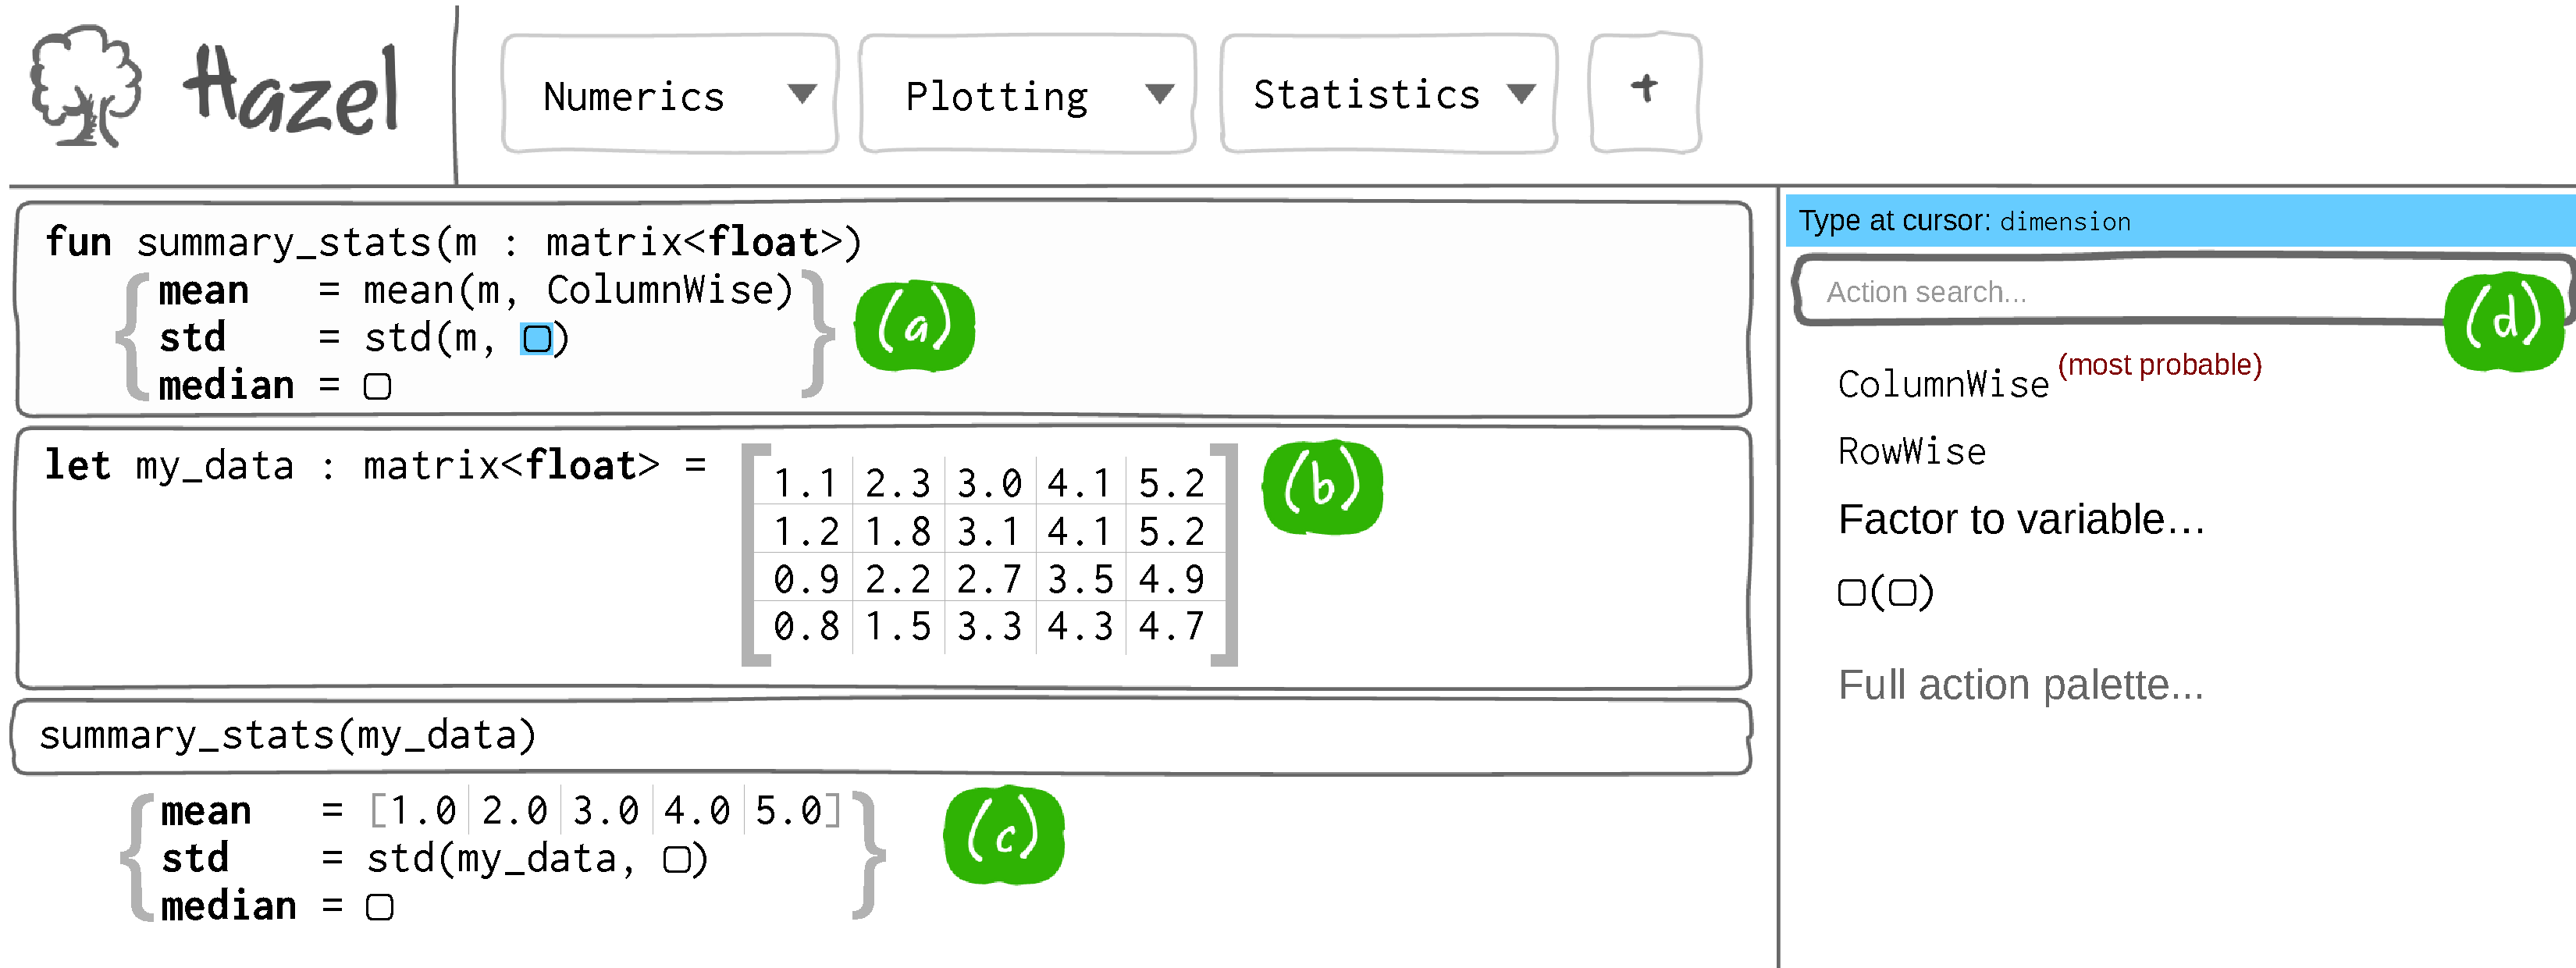
\includegraphics[width=1.025\textwidth]{mockup-1}
\caption{A mockup of \HazelEnv.}
\label{fig:hazel-mockup}
%\vspace{-2ex}
\end{figure}

\paragraph{Problem 2: Statically Meaningless Edit States.} Regardless of how an 
editor confronts syntactically malformed edit states, it must also confront 
edit states that are syntactically well-formed but statically meaningless. For
example, the following value binding has a type inconsistency:
\begin{lstlisting}[numbers=none]
val x : string = std(m, ColumnWise)
\end{lstlisting}
(because \li{std} has type \li{matrix<float> * dimension -> vec<float>},
but the type annotation on \li{x} is \li{string}.) This leaves the entire program
formally meaningless according to a standard static semantics.

In the presence of holes, the problem of reasoning statically about edit states
becomes even more interesting.  Consider the incomplete expression \lstinline{std(m, #$\square$#)} 
from cell \textbf{(a)} in Figure \ref{fig:hazel-mockup}.
%
%\begin{lstlisting}[numbers=none]
%std(m, #$\square$#)
%\end{lstlisting}
%
Although it is apparent that the type of this expression, after hole instantiation, could only be \lstinline{vec<float>} (the return type of \lstinline{std}),
and that the hole must be instantiated with values of type \li{dimension}, the static
semantics of complete expressions is again silent about these matters. 

Various heuristic
approaches are implemented in Eclipse and other sophisticated tools, but the 
formal character of these heuristics are obscure, buried deep within their implementations. This brings us to our first specific research aim: the 
development, from type-theoretic first principles, of \textbf{a static semantics for incomplete programs} (Section~\ref{sec:statics}),
i.e. programs that contain holes, type inconsistencies, unbound variables, and
other static problems. Using such a semantics, \HazelEnv can 
communicate to the programmer (see right column of Figure \ref{fig:hazel-mockup}) that the expression at the cursor, highlighted in blue in cell \textbf{(a)}, must be of type \li{dimension}. The incomplete function
\li{summary_stats} as a whole will be assigned the following incomplete function
type: \texttt{matrix<float> -> \{ {mean} : vec<float>, std : vec<float>, median :~$\square$ \}}.

\paragraph{Problem 3: Dynamically Meaningless Edit States.} Modern programming
tools are increasingly moving beyond simple ``batch'' programming models by
incorporating \emph{live programming} features that interleave editing and
evaluation \cite{DBLP:conf/icse/Tanimoto13,DBLP:journals/vlc/Tanimoto90,McDirmid:2007:LUL:1297105.1297073}. These tools provide programmers with more rapid feedback about the
dynamic behavior of the program they are editing, or selected portions thereof \cite{McDirmid:2013:ULP:2509578.2509585}. Examples include \emph{lab notebooks},
e.g. the popular IPython/Jupyter~\cite{Perez:2007:ISI:1251563.1251831}, which allow the
programmer to interactively edit and evaluate program fragments organized into a
sequence of cells (an extension of the read-eval-print loop (REPL)); spreadsheets; {live graphics programming environments}, e.g. SuperGlue \cite{McDirmid:2007:LUL:1297105.1297073}, Sketch-n-Sketch \cite{DBLP:conf/pldi/ChughHSA16,DBLP:conf/icse/Chugh25} and the tools demonstrated by Bret Victor in his lectures \cite{victor2012inventing}; the TouchDevelop live UI framework \cite{burckhardt2013s}; and live visual and auditory dataflow languages \cite{DBLP:conf/vl/BurnettAW98}. 
% \item \emph{Live debuggers} allow the programmer to:
%   \begin{itemize}
%   \item insert breakpoints, which pause evaluation; 
%   \item step through evaluation one step at a time; 
%   \item inspect the run-time state of a paused program by ``watching'' expressions; and 
%   \item edit the program and resume evaluation in certain circumstances. 
%   \end{itemize}

Our proposed design for \HazelEnv combines aspects of several of these designs to form a \emph{live lab notebook interface}. 
It will use the edit state of each cell to continuously update the output
value displayed for that cell and subsequent cells that depend on
it. Uniquely, rather than providing meaningful feedback about the dynamic
behavior only once a cell becomes complete, \HazelEnv will provide meaningful feedback also
about the dynamic behavior of incomplete cells (and thereby further tighten the live programming 
feedback loop.)

For example, in cell \textbf{(c)} of Figure~\ref{fig:hazel-mockup}, the
programmer applies  the incomplete function \li{summary_stats} to 
the matrix \lstinline{my_data}, and 
the editor is still able to display a result.
The value of the column-wise mean is fully determined, because evaluation does
not encounter any holes, whereas the standard deviation and median computations
cannot be fully evaluated. Notice, however, that the standard
deviation computation does communicate the substitution of the applied argument,
\li{my_data}, for the variable \li{m}.\footnote{To avoid exposing the internals
of imported library functions, evaluation does not step into functions, like
\li{std}, that have been imported from external libraries indicated by the row at the top of Figure \ref{fig:hazel-mockup} (unless specifically
requested, not shown.)}

This brings us to our second specific aim: a
\textbf{dynamic semantics for incomplete programs} (Section~\ref{sec:dynamics}) that builds upon our proposed
static semantics. There is some precedent for this: research in gradual typing
considers the dynamic semantics of programs with holes in types, and indeed, our
proposed static semantics for incomplete programs borrows technical machinery
from theoretical work on gradual typing~\cite{Siek06a}. We seek a dynamic semantics for the
other classes of incomplete programs that we will consider as well.

This will require great formal care, because the presence of type
and binding errors would violate the usual notions of type safety. As such we plan to develop a \emph{mechanized
  metatheory}~\cite{Lee:2007:TMM:1190216.1190245}: we will use a proof assistant to mechanize the semantics and
accompanying metatheorems that establish essential properties, e.g. that
evaluating a statically meaningful incomplete programs will not ``go wrong'' (which we take in
the sense of Milner to mean that it will not have undefined behavior~\cite{milner1978theory,pfpl}).
This represents the ``gold standard'' for evaluating claims in formal
semantics.  Our preliminary work has used Agda~\cite{norell2009dependently}.

\paragraph{Problem 4: Meaningless Edit Actions.} Our first two specific aims
allow us to assign meaning to intermediate edit states. However, to
understand the act of \emph{editing} itself, we propose to develop a system of
\emph{edit actions} that governs transitions between edit
states. Our goal is for every intermediate edit state to be both statically and
dynamically meaningful according to the semantics developed in the first two
specific aims. This corresponds formally to proving a
metatheorem about the action semantics: when the initial edit state is
semantically meaningful, the edit state that results from performing an action
is as well. In addition to this crucial metatheorem, which
we call \emph{sensibility}, there are a number of other metatheorems of interest
that establish the interactive expressive power of the action semantics. Our third specific
aim is thus to develop a sensible and expressive \textbf{semantics of edit actions} (Section~\ref{sec:actions})
and, as above, to mechanize its metatheory.

Designing the static semantics of \HazelEnv together with its action semantics 
will also allow us to rigorously investigate a number of novel constructs that 
are defined with libraries but control aspects of the editor. In particular, we aim to explore:
(1) \textbf{user-defined action macros}, which allow libraries to define new high-level
actions built atop the primitive action language of \HazelEnv; (2) \textbf{type-specific
projections}, which give library providers the ability to define type-specific structure editors (e.g. the matrix interface in Figure \ref{fig:hazel-mockup}, which is defined  
by the \li{Numerics} library); and (3) an \textbf{interactive semantic documentation system} that
allows programmers to document programs by revealing and commenting on portions of the 
program in sequence. Each intermediate state during these ``tutorials'' can be explored 
by the learner, due to the sensibility invariant. The comments can mention bindings, and are 
subject to static operations like renaming.

\paragraph{Problem 5: Meaningless and Improbable Suggestions.} The simplest 
edit actions will be bound to keyboard shortcuts (studies suggest that programmers experienced with a keyboard-driven structure editors can be highly productive \cite{DBLP:conf/vl/Asenov014}). However, \HazelEnv will 
also present a search-based user
interface for discovering relevant higher-level actions -- marked with \textbf{(d)} in Figure \ref{fig:hazel-mockup}. 
The suggestions 
listed are informed by the semantics at the cursor, i.e. they use the fact that
the type at the cursor is \li{dimension} to suggest the two constructors of that
type, \li{ColumnWise} and \li{RowWise}. The suggestions are further informed by
the statistics of other programs that \HazelEnv has encountered.  Here, the
environment has noticed that the programmer tends to prefer column-wise operations on 
matrices, so it marks that suggestion as the most probable. These suggestions are governed by
our fourth specific aim: a \textbf{statistical action suggestion semantics} (Section~\ref{sec:statistics}). The key invariant here that, again, we aim to establish 
formally is that every suggestion assigned non-zero probability must be semantically sensible 
relative to the edit state.% Moreover, all probability distributions must ``integrate'' to $1$.

\paragraph{Roadmap.} Sections~\ref{sec:statics}--\ref{sec:statistics} detail the
specific aims mentioned above; our evaluation plan is discussed in Section~\ref{sec:eval}.
The collaboration plan details our 
research timeline, and the relevant qualifications of the PIs.

% To summarize, 
% the following are the specific aims of the proposed reasearch.

% \begin{enumerate}[labelwidth=0.7em, labelsep=0.6em, topsep=0ex, itemsep=0ex,
%   parsep=0ex]
% \item A static semantics for incomplete programs (Section~\ref{sec:statics}).
% \item A dynamic semantics for incomplete programs (Section~\ref{sec:dynamics}).
% \item An edit action semantics (Section~\ref{sec:actions})
% \item Statistical program inferene semantics (Section~\ref{sec:statistics})
% \item \HazelEnv, an integrated interactive programming environment (Section~\ref{sec:hazel})

% \end{enumerate}

% !TEX root = hazelnut-popl17.tex

% Violet hotdogs; highlight color helps distinguish them
\newcommand{\llparenthesiscolor}{\textcolor{violet}{\llparenthesis}}
\newcommand{\rrparenthesiscolor}{\textcolor{violet}{\rrparenthesis}}

% HTyp and HExp
\newcommand{\hcomplete}[1]{#1~\mathsf{complete}}

% HTyp
\newcommand{\htau}{\dot{\tau}}
\newcommand{\tarr}[2]{#1 \rightarrow #2}
\newcommand{\tnum}{\texttt{num}}
\newcommand{\tehole}{\llparenthesiscolor\rrparenthesiscolor}
\newcommand{\tsum}[2]{{#1} + {#2}}

\newcommand{\tcompat}[2]{#1 \sim #2}
\newcommand{\tincompat}[2]{#1 \nsim #2}

% HExp
\newcommand{\hexp}{\dot{e}}
\newcommand{\hlam}[2]{\lambda #1.#2}
\newcommand{\hap}[2]{#1(#2)}
\newcommand{\hapP}[2]{(#1)~(#2)} % Extra paren around function term
\newcommand{\hnum}[1]{\underline{#1}}
\newcommand{\hadd}[2]{#1 + #2}
\newcommand{\hehole}{\llparenthesiscolor\rrparenthesiscolor}
\newcommand{\hhole}[1]{\llparenthesiscolor#1\rrparenthesiscolor}
\newcommand{\hindet}[1]{\lceil#1\rceil}
\newcommand{\hinj}[2]{\texttt{inj}_{#1}({#2})}
\newcommand{\hcase}[5]{\texttt{case}({#1},{#2}.{#3},{#4}.{#5})}

\newcommand{\hGamma}{\dot{\Gamma}}
\newcommand{\domof}[1]{\text{dom}(#1)}
\newcommand{\hsyn}[3]{#1 \vdash #2 \Rightarrow #3}
\newcommand{\hana}[3]{#1 \vdash #2 \Leftarrow #3}

% ZTyp and ZExp
\newcommand{\zlsel}[1]{{\bowtie}{#1}}
\newcommand{\zrsel}[1]{{#1}{\bowtie}}
\newcommand{\zwsel}[1]{
  \setlength{\fboxsep}{0pt}
  \colorbox{green!10!white!100}{
    \ensuremath{{{\textcolor{Green}{{\hspace{-2px}\triangleright}}}}{#1}{\textcolor{Green}{\triangleleft{\vphantom{\tehole}}}}}}
}

\newcommand{\removeSel}[1]{#1^{\diamond}}

% ZTyp
\newcommand{\ztau}{\hat{\tau}}

% ZExp
\newcommand{\zexp}{\hat{e}}

% Direction
\newcommand{\dParent}{\mathtt{parent}}
\newcommand{\dChildn}[1]{\mathtt{child}~\mathtt{{#1}}}
\newcommand{\dChildnm}[1]{\mathtt{child}~{#1}}

% Action
\newcommand{\aMove}[1]{\mathtt{move}~#1}
	\newcommand{\zrightmost}[1]{\mathsf{rightmost}(#1)}
	\newcommand{\zleftmost}[1]{\mathsf{leftmost}(#1)}
\newcommand{\aSelect}[1]{\mathtt{sel}~#1}
\newcommand{\aDel}{\mathtt{del}}
\newcommand{\aReplace}[1]{\mathtt{replace}~#1}
\newcommand{\aConstruct}[1]{\mathtt{construct}~#1}
\newcommand{\aConstructx}[1]{#1}
\newcommand{\aFinish}{\mathtt{finish}}

%% \newcommand{\performAna}[5]{#1 \vdash #2 \xlongrightarrow{#4} #5 \Leftarrow #3}
%% \newcommand{\performAnaI}[5]{#1 \vdash #2 \xlongrightarrow{#4}\hspace{-3px}{}^{*}~ #5 \Leftarrow #3}
%% \newcommand{\performSyn}[6]{#1 \vdash #2 \Rightarrow #3 \xlongrightarrow{#4} #5 \Rightarrow #6}
%% \newcommand{\performSynI}[6]{#1 \vdash #2 \Rightarrow #3 \xlongrightarrow{#4}\hspace{-3px}{}^{*}~ #5 \Rightarrow #6}
%% \newcommand{\performTyp}[3]{#1 \xlongrightarrow{#2} #3}
%% \newcommand{\performTypI}[3]{#1 \xlongrightarrow{#2}\hspace{-3px}{}^{*}~#3}

%% \newcommand{\performMove}[3]{#1 \xlongrightarrow{#2} #3}
%% \newcommand{\performDel}[2]{#1 \xlongrightarrow{\aDel} #2}

\newcommand{\performAna}[5]{#1 \vdash #2 \xrightarrow{#4} #5 \Leftarrow #3}
\newcommand{\performAnaI}[5]{#1 \vdash #2 \xrightarrow{#4}\hspace{-3px}{}^{*}~ #5 \Leftarrow #3}
\newcommand{\performSyn}[6]{#1 \vdash #2 \Rightarrow #3 \xrightarrow{#4} #5 \Rightarrow #6}
\newcommand{\performSynI}[6]{#1 \vdash #2 \Rightarrow #3 \xrightarrow{#4}\hspace{-3px}{}^{*}~ #5 \Rightarrow #6}
\newcommand{\performTyp}[3]{#1 \xrightarrow{#2} #3}
\newcommand{\performTypI}[3]{#1 \xrightarrow{#2}\hspace{-3px}{}^{*}~#3}

\newcommand{\performMove}[3]{#1 \xrightarrow{#2} #3}
\newcommand{\performDel}[2]{#1 \xrightarrow{\aDel} #2}

% Form
\newcommand{\farr}{\mathtt{arrow}}
\newcommand{\fnum}{\mathtt{num}}
\newcommand{\fsum}{\mathtt{sum}}

\newcommand{\fasc}{\mathtt{asc}}
\newcommand{\fvar}[1]{\mathtt{var}~#1}
\newcommand{\flam}[1]{\mathtt{lam}~#1}
\newcommand{\fap}{\mathtt{ap}}
% \newcommand{\farg}{\mathtt{arg}}
\newcommand{\fnumlit}[1]{\mathtt{lit}~#1}
\newcommand{\fplus}{\mathtt{plus}}
\newcommand{\fhole}{\mathtt{hole}}
\newcommand{\fnehole}{\mathtt{nehole}}

\newcommand{\finj}[1]{\mathtt{inj}~#1}
\newcommand{\fcase}[2]{\mathtt{case}~#1~#2}

% Talk about formal rules in example
\newcommand{\refrule}[1]{\textrm{Rule~(#1)}}

\newcommand{\herase}[1]{\left|#1\right|_\textsf{erase}}

\newcommand{\arrmatch}[2]{#1 \blacktriangleright_{\rightarrow} #2}


\newcommand{\TABperformAna}[5]{#1 \vdash & #2                & \xrightarrow{#4} & #5 & \Leftarrow #3}
\newcommand{\TABperformSyn}[6]{#1 \vdash & #2 \Rightarrow #3 & \xrightarrow{#4} & #5 \Rightarrow #6}
\newcommand{\TABperformTyp}[3]{& #1 & \xrightarrow{#2} & #3}

\newcommand{\TABperformMove}[3]{#1 & \xrightarrow{#2} & #3}
\newcommand{\TABperformDel}[2]{#1 \xrightarrow{\aDel} #2}

\newcommand{\sumhasmatched}[2]{#1 \mathrel{\textcolor{black}{\blacktriangleright_{+}}} #2}

\newcommand{\subminsyn}[1]{\mathsf{submin}_{\Rightarrow}(#1)}
\newcommand{\subminana}[1]{\mathsf{submin}_{\Leftarrow}(#1)}

% !TEX root = prop.tex
%\clearpage
\section{Aim 1: A Static Semantics for Incomplete Programs}\label{sec:statics}
\vspace{-3px}

Incomplete programs are programs that contain (1) holes, signifying leaves of the syntax tree that have not yet been constructed, (2) type inconsistencies, or (3) binding inconsistencies
(e.g. unbound variables). Incomplete programs are meaningless from the
perspective of a standard static semantics. Our intuition is that
these problems are \emph{local}, so they should be \emph{localized} and not render the entire program statically meaningless. This, in turn, will allow  
\HazelEnv to support editor services that rely on a formal understanding of the type
and binding structure of every edit state.

\subsection{Preliminary Work}

\begin{figure}[t]
%\small
$\arraycolsep=4pt\begin{array}{lllllll}
\mathsf{HTyp:} & \htau & ::= &
  \tarr{\htau}{\htau} ~\vert~
  \tnum ~\vert~
  \tehole
\\
\mathsf{HExp:} & \hexp & ::= &
  x ~\vert~
  \hlam{x}{\hexp} ~\vert~
  \hap{\hexp}{\hexp} ~\vert~
  \hnum{n} ~\vert~
  \hadd{\hexp}{\hexp} ~\vert~
  (\hexp : \htau) ~\vert~
  \hehole ~\vert~
  \hhole{\hexp}
\end{array}$
\caption{Syntax of H-types and H-expressions. Metavariable $x$ ranges over variables and $n$ over numerals.}
\label{fig:hexp-syntax}
\vspace{-5px}
\end{figure}


Partially in preparation for this proposal, we conducted preliminary research to define a static
semantics for a simply typed lambda calculus (with a 
single base type, $\tnum$, for simplicity) extended with holes and type
inconsistencies, but no binding inconsistencies (the results summarized below are detailed in a paper accepted at POPL 2017 \cite{popl-paper}). Figure~\ref{fig:hexp-syntax} defines the syntactic
objects of this calculus -- \emph{H-types}, $\htau$,
are types with holes $\tehole$, and \emph{H-expressions}, $\hexp$, are
expressions with holes $\hehole$, and marked type inconsistencies,
$\hhole{\hexp}$. We call marked type inconsistencies \emph{non-empty holes},
because they mark portions of the syntax tree that remain
incomplete and, as we will see, behave semantically much like empty holes. Types and expressions that contain no holes are \emph{complete
  types} and \emph{complete expressions}, respectively.


\begin{figure}%{r}{0.35\textwidth}
%\small
\footnotesize
\begin{subequations}
\fbox{$\hsyn{\hGamma}{\hexp}{\htau}$}~~\text{$\hexp$ synthesizes $\htau$}
\begin{equation}\label{rule:syn-var}
\inferrule{ }{
  \hsyn{\hGamma, x : \htau}{x}{\htau}
}
\end{equation}
\begin{equation}\label{rule:syn-ap}
\inferrule{
  \hsyn{\hGamma}{\hexp_1}{\htau}\\
  \arrmatch{\htau}{\tarr{\htau_2}{\htau'}}\\
  \hana{\hGamma}{\hexp_2}{\htau_2}
}{
  \hsyn{\hGamma}{\hap{\hexp_1}{\hexp_2}}{\htau'}
}
\end{equation}
\begin{equation}\label{rule:syn-num}
\inferrule{ }{
  \hsyn{\hGamma}{\hnum{n}}{\tnum}
}
\end{equation}
\begin{equation}\label{rule:syn-plus}
\inferrule{
  \hana{\hGamma}{\hexp_1}{\tnum}\\
  \hana{\hGamma}{\hexp_2}{\tnum}
}{
  \hsyn{\hGamma}{\hadd{\hexp_1}{\hexp_2}}{\tnum}
}
\end{equation}
\begin{equation}\label{rule:syn-asc}
\inferrule{
  \hana{\hGamma}{\hexp}{\htau}
}{
  \hsyn{\hGamma}{(\hexp : \htau)}{\htau}
}
\end{equation}
\begin{equation}\label{rule:syn-ehole}
\inferrule{ }{
  \hsyn{\hGamma}{\hehole}{\tehole}
}
\end{equation}
\begin{equation}\label{rule:syn-hole}
\inferrule{
  \hsyn{\hGamma}{\hexp}{\htau}
}{
  \hsyn{\hGamma}{\hhole{\hexp}}{\tehole}
}
\end{equation}
\end{subequations}
\fbox{$\hana{\hGamma}{\hexp}{\htau}$}~~\text{$\hexp$ analyzes against $\htau$}
\begin{subequations}
\begin{equation}\label{rule:ana-subsume}
\inferrule{
  \hsyn{\hGamma}{\hexp}{\htau'}\\
  \tcompat{\htau}{\htau'}
}{
  \hana{\hGamma}{\hexp}{\htau}
}
\end{equation}
\begin{equation}\label{rule:syn-lam}
\inferrule{
  \arrmatch{\htau}{\tarr{\htau_1}{\htau_2}}\\
  \hana{\hGamma, x : \htau_1}{\hexp}{\htau_2}
}{
  \hana{\hGamma}{\hlam{x}{\hexp}}{\htau}
}
\end{equation}
\end{subequations}
\vspace{-5px}
\caption{The bidirectional H-typing rules for incomplete expressions.\label{fig:ana-synth}}
\end{figure}
We define the static semantics of H-types and H-expressions as a \emph{bidirectional type
  system}~\cite{Pierce:2000:LTI:345099.345100,DBLP:conf/icfp/DaviesP00,DBLP:conf/tldi/ChlipalaPH05,bidi-tutorial}
around the two mutually defined judgements in Figure~\ref{fig:ana-synth}. Typing contexts, $\hGamma$, map each variable $x \in
\domof{\hGamma}$ to a hypothesis $x : \htau$ in the usual manner. 
%
Derivations of the type analysis judgement, $\hana{\hGamma}{\hexp}{\htau}$,
establish that $\hexp$ can appear where an expression of type $\htau$ is
expected. Derivations of the type synthesis judgement,
$\hsyn{\hGamma}{\hexp}{\htau}$, infer a type from $\hexp$, which is
necessary in positions where an expected type is not available (e.g. at the
top level.) Algorithmically, the type is an ``input'' of the type analysis
judgement, but an ``output'' of the type synthesis judgement.  Making a
judgemental distinction between these two situations is essential in our
action semantics (Section~\ref{sec:actions}).

Type synthesis is stronger than type analysis in that if an expression is
able to synthesize a type, it can also be analyzed against that type, or
any other \emph{consistent} type, according to the \emph{subsumption rule},
Rule (\ref{rule:ana-subsume}). The \emph{H-type consistency judgement}, $\tcompat{\htau}{\htau'}$, that
appears as a premise in the subsumption rule is a reflexive and symmetric
(but not transitive) relation between H-types defined judgementally in
Figure \ref{fig:type-consistency}. This relation coincides with equality
for complete H-types. Two incomplete H-types are consistent if they differ
only at positions where a hole appears in either type. The type hole is
therefore consistent with every type. This notion of H-type consistency
coincides with the notion of type consistency that Siek and Taha discovered
in their foundational work on gradual type systems, if we interpret the
type hole as the $?$ (i.e. unknown) type \cite{Siek06a}. This discovery is quite encouraging, given that gradual typing is also motivated by a 
desire to make sense of one class of ``intermediate edit states,'' or programs that
have not yet been fully annotated with types.

Rule (\ref{rule:syn-lam}) defines analysis for lambda abstractions,
$\hlam{x}{\hexp}$. There is no type synthesis rule that applies  
to this form, so lambda abstractions can appear only in analytic position,
i.e. where an expected type is known.\footnote{It is possible to also define a
  ``half-annotated'' synthetic lambda form, $\lambda x{:}\tau.e$, but for
  simplicity, we leave it out \cite{DBLP:conf/tldi/ChlipalaPH05}.}  Rule
(\ref{rule:syn-lam}) is not quite the standard rule,
%
% CLG says we don't have room 
% reproduced below:
% \begin{equation*}
% \inferrule{
%   \hana{\hGamma, x : \htau_1}{\hexp}{\htau_2}
% }{
%   \hana{\hGamma}{\hlam{x}{\hexp}}{\tarr{\htau_1}{\htau_2}}
% }
% \end{equation*}
which on its own would leave us unable to analyze
lambda abstractions against the type hole.
%because the type hole is not
%immediately of the form $\tarr{\htau_1}{\htau_2}$. 
Although we could solve this problem by defining a rule 
specifically for that case, we 
% \begin{equation*}
% \inferrule{
%   \hana{\hGamma, x : \tehole}{\hexp}{\tehole}
% }{
%   \hana{\hGamma}{\hlam{x}{\hexp}}{\tehole}
% }
% \end{equation*}
instead produce a single rule through the
simple auxiliary \emph{matched arrow type} judgement,
$\arrmatch{\htau}{\tarr{\htau_1}{\htau_2}}$, defined in Figure
\ref{fig:type-consistency}. This judgement leaves arrow types alone and
assigns the type hole the matched arrow type $\tarr{\tehole}{\tehole}$.  
Rule (\ref{rule:syn-ap}), which governs function
application, also makes use of the matched arrow type judgement to
combine what would otherwise need to be two rules for function application:
one for when $e_1$ synthesizes an arrow type, and another for when $e_1$
synthesizes the type hole. Indeed, Siek and Taha needed two application
rules for the same fundamental reason~\cite{Siek06a}. Later work on gradual
typing introduced this notion of type matching to resolve this redundancy \cite{DBLP:conf/popl/CiminiS16,DBLP:conf/popl/GarciaC15,DBLP:conf/popl/RastogiCH12}.

% Rule (\ref{rule:syn-num}) states that numbers synthesize the $\tnum$
% type. Rule (\ref{rule:syn-plus}) states that $\hexp_1 + \hexp_2$ behaves
% like a function over numbers.
% %
% Rule (\ref{rule:syn-asc}) defines type synthesis of expressions of
% ascription form, $\hexp : \htau$. This allows the user to explicitly state
% a type for the ascribed expression to be analyzed against.

% %
% The rules described so far are sufficient to type complete
% H-expressions. The two remaining rules give H-expressions with holes a
% well-defined static semantics. 


\begin{figure}%{l}{0.5\textwidth}
%\small
\footnotesize
\noindent\fbox{$\tcompat{\htau}{\htau'}$}~~\text{$\htau$ and $\htau'$ are consistent}
\begin{subequations}\label{eqns:consistency}
\begin{mathpar}
\inferrule{ }{
  \tcompat{\tehole}{\htau}
}

\inferrule{ }{
  \tcompat{\htau}{\tehole}
}

\inferrule{ }{
  \tcompat{\htau}{\htau}
}

\inferrule{
  \tcompat{\htau_1}{\htau_1'}\\
  \tcompat{\htau_2}{\htau_2'}
}{
  \tcompat{(\tarr{\htau_1}{\htau_2})}{(\tarr{\htau_1'}{\htau_2'})}
}
\end{mathpar}
\end{subequations}
\fbox{$\arrmatch{\htau}{\tarr{\htau_1}{\htau_2}}$}~~\text{$\htau$ has matched arrow type $\tarr{\htau_1}{\htau_2}$}
\begin{subequations}
\begin{mathpar}
\inferrule{ }{
  \arrmatch{\tarr{\htau_1}{\htau_2}}{\tarr{\htau_1}{\htau_2}}
}

\inferrule{ }{
  \arrmatch{\tehole}{\tarr{\tehole}{\tehole}}
}
\end{mathpar}
\end{subequations}
\caption{H-type consistency; matched arrow types.}
\label{fig:type-consistency}
\end{figure}
Gradual type systems do not consider holes in expression position. Rule (\ref{rule:syn-ehole}) states that the empty expression hole
synthesizes the type hole. Similarly, according to Rule
(\ref{rule:syn-hole}), non-empty holes also synthesize the hole type, as long as the inner H-expression  synthesizes some type. By the subsumption rule and the definition of type consistency, holes can be analyzed against any type.

% CLG this is really informative but just takes too much space.
Given these rules, it is instructive to derive that $\hana{incr : \tarr{\tnum}{\tnum}}{\hhole{incr}}{\tnum}$. 
That is, the function variable $incr$ can appear where an expression of number type is needed, as long as the type inconsistency has been marked. Non-empty holes can be used in this way to internalize the ``squiggly red lines'' that many editors display under type inconsistencies. 

The simple static semantics just described has been mechanized using the Agda proof assistant. It serves as the statics for Hazelnut, a structure editor calculus that we return to in Section~\ref{sec:actions}.

\subsection{Proposed Research}

\noindent\textbf{Binding inconsistencies.} In the simple calculus developed so far,
    all variables must be bound before they are used,
    including those in holes. We will extend this system to support reasoning
    in the presence of binding inconsistencies. This 
    opens a new class of type inconsistencies: an unbound variable
    might be used in several places with different, inconsistent types. Tracking
    the types of unbound variables will therefore require tracking and solving typing constraints.  Dagenais and
    Hendren also studied how to reason statically about programs
    with binding errors using a constraint system, focusing on
    Java programs whose imports are not completely known~\cite{DBLP:conf/oopsla/DagenaisH08}. They neither
    considered programs with holes or other type inconsistencies,
    nor formally mathematically specificied their
    technique. However, they provide a useful starting point for us.

\vspace{0.25ex} 
\noindent\textbf{Practical extensions.} The simple calculus
    is only as expressive as the typed lambda calculus with numbers. We have further investigated,
    as an exercise, an extension with binary sum
    types. We propose to scale up the semantics to handle other modern language
    features, focusing initially on functional language
    constructs (so that \HazelEnv can be used to teach courses that
    are today taught using Standard ML, OCaml or Haskell.) This will include recursive and
    polymorphic functions, recursive types, and labeled product (record) and sum types.
    We also propose to investigate ML-style structural pattern
    matching. All of these will require defining new sorts of holes and static
    inconsistencies, including: (1) non-empty holes at the type level, to handle
    kind inconsistencies; (2) holes in label position; (3) label inconsistency
    errors; and (4) holes and type inconsistencies in patterns. 

\vspace{0.25ex} 
\noindent\textbf{Automation.} Although we plan to
    explore some of these language extensions 
    ``manually,'' extending our existing mechanization, we ultimately plan 
    to \emph{automatically}
    generate a statics for incomplete terms from a standard statics for complete terms,
    annotated perhaps with additional information. There is some precedent for
    this in recent work on the Gradualizer, which is capable of
    producing a gradual type system from a standard type system with lightweight
    annotations that communicate the intended polarities of certain
    constructs~\cite{DBLP:conf/popl/CiminiS16}. However, although it provides a good starting point, gradual type systems 
    only consider the problem of holes in 
    types, and the Gradualizer does not support bidirectionally typed languages.
    Our plan is to build 
    upon existing proof automation techniques, e.g. Agda's reflection \cite{van2012engineering}.


% !TEX root = prop.tex
%\clearpage

\definecolor{dRed}{rgb}{0.65, 0.0, 0.0}
\definecolor{dDkRed}{rgb}{0.35, 0.0, 0.0}
\definecolor{dLighterGreen}{rgb}{0.70, 0.95, 0.70}
\definecolor{dGreen}{rgb}{0.0, 0.65, 0.0}
\definecolor{dDkGreen}{rgb}{0.0, 0.35, 0.0}
\definecolor{dBlue}{rgb}{0.0, 0.0, 0.65}
\definecolor{dLightBlue}{rgb}{0.4, 0.4, 0.9}
\definecolor{dLighterBlue}{rgb}{0.8, 0.8, 1.0}
\definecolor{dDkBlue}{rgb}{0.0, 0.0, 0.45}
\definecolor{dLightPurple}{rgb}{0.9, 0.5, 0.9}
\definecolor{dLighterPurple}{rgb}{1.0, 0.7, 1.0}
\definecolor{dPurple}{rgb}{0.65, 0.0, 0.65}
\definecolor{dDigPurple}{rgb}{0.5, 0.0, 0.5}
% \definecolor{DDIGPURPLE}{rgb}{0.5, 0.0, 0.5}  % laughable
\definecolor{dFaint}{rgb}{0.7, 0.7, 0.7}
\definecolor{dVeryFaint}{rgb}{0.9, 0.9, 0.9}
\definecolor{dGray}{rgb}{0.5, 0.5, 0.5}
\definecolor{dDark}{rgb}{0.2, 0.2, 0.2}
\definecolor{dAlmostBlack}{rgb}{0.1, 0.1, 0.1}
\definecolor{lred}{rgb}{1.0, 0.8, 0.8}
\definecolor{white}{rgb}{1.0, 1.0, 1.0}

\newcommand{\OmitThis}[1]{}
\newcommand{\metavar}[0]{u}

%Matt's hole macro
%\newcommand{\mhole}[1]{%
%{\color{dPurple}(\!|}%
%{#1}%
%{\color{dPurple}|\!)}%
%}
%\newcommand{\mhole}[1]{\colorbox{dPurple}{\colorbox{white}{\ensuremath{#1}}}}
\newcommand{\mhole}[1]{\hehole}
\newcommand{\indet}[1]{\lfloor{#1}\rfloor}
\newcommand{\desc}[1]{\textrm{#1}}
%% \newcommand{\testaction}[1]{\colorbox{dLighterGreen}{\ensuremath{#1}}}
%% \newcommand{\editaction}[1]{\colorbox{dLighterPurple}{\ensuremath{#1}}}
%% \newcommand{\editreaction}[1]{\colorbox{dLightPurple}{\ensuremath{#1}}}
%% \newcommand{\indetaction}[1]{\colorbox{dFaint}{\ensuremath{#1}}}
%% \newcommand{\detaction}[1]{\colorbox{dLightPurple}{\ensuremath{#1}}}
%% \newcommand{\stepaction}[1]{\colorbox{dLighterBlue}{#1}}
\newcommand{\testaction}[1]{\ensuremath{#1}}
\newcommand{\editaction}[1]{\ensuremath{#1}}
\newcommand{\editreaction}[1]{\ensuremath{#1}}
\newcommand{\indetaction}[1]{\ensuremath{#1}}
\newcommand{\detaction}[1]{\ensuremath{#1}}
\newcommand{\stepaction}[1]{{#1}}
\newcommand{\ScenerioOne}{Scenario 1\xspace}
\newcommand{\ScenerioOneA}{Scenario 1(a)\xspace}
\newcommand{\ScenerioOneB}{Scenario 1(b)\xspace}
\newcommand{\ScenerioTwo}{Scenario 2\xspace}
\newcommand{\Pass}{\colorbox{dLighterBlue}{P}}
\newcommand{\Fail}{\colorbox{lred}{F}}
\newcommand{\Indet}{\colorbox{dFaint}{I}}


\section{Aim 2: A Dynamic Semantics for Incomplete Programs}
\label{sec:dynamics}

Broadly speaking, live programming environments interleave editing and evaluation. 
Several examples were listed in Section \ref{sec:objectives}, and indeed many more
are under development. In the words of Burckhardt et al., live programming environments 
``capture the imagination of today's programmers and promise to narrow the temporal and perceptive gap 
between program development and code execution'' \cite{burckhardt2013s}. However,
contemporary live programming environments are typically equipped only to provide feedback once the program or 
program fragment being evaluated is complete. This leaves a temporal and perceptive gap. Listing \ref{fig:hazel-mockup} showed an example where
useful information---the column-wise mean---can be extracted from an incomplete program, even though a final value cannot be computed. It is not difficult to imagine other such scenarios.

The second specific aim of this proposal is to develop a semantics that characterizes exactly how
evaluation of an incomplete program should proceed. A related semantic question (which is also of 
substantial practical relevance) has to do with how 
evaluation and editing interact: it should, ideally, be possible to avoid restarting
evaluation ``from scratch'' after every edit to the program.

%% \todo{It would be nice if we could more explicitly separate
%% out concrete research objectives from the overview, to lay it out
%% really simply for the reader.  CLG is having a hard time detangling
%% them; perhaps Matt or Cyrus could try?}

%
%In particular, the programmer uses this interface to edit the
%expression that they are running, while making edits ``retroactive''
%when they choose to do so.
%
% CLG says:  I think that the multiple levels of intro to the idea by pointing
% to the Hazel mockup and walking through the scenarios is really helpful for
% clarity.  BUT we also don't have room for them, and so I made the executive
% decision to keep the code 
% For example, in Figure~\ref{fig:hazel-mockup}, cells~$a$ and~$c$ are related by
% evaluation.
% %
% Cell~$a$ defines an incomplete function, \texttt{summary\_stats}, and
% cell~$c$ shows the call for and result of invoking this function on a
% concrete input, the matrix constant defined in cell~$b$.
% %
% This result in cell~$c$ is \emph{incomplete} since it
% depends on an incomplete function in cell~$a$.
% %
% Suppose that the programmer wants to finish this program by using
% dynamic information that is kept ``live'', or up-to-date, with the
% program as they edit.  In particular, they wish to mix
% editing these holes with the live relationship between cells~$a$
% and~$c$, where the latter is the output of running the former.
%
% First, notice that in cell~$c$, the hole in field~\texttt{std} can be
% attributed uniquely to the field~\texttt{std} hole in cell~$a$.
% %
% This is an instance of a more general property that we refer to
% as \textbf{hole provenance}.
% %
% Suppose that the user edits this hole, choosing to enter the abstract
% constant \texttt{ColumnWise}.
% %
% We can imagine this interacting with evaluation in one of two ways:
% First, we imagine editing the hole in cell~$c$, and permitting
% cell~$c$ to evaluate further, to produce, say, cell~$d$ (not shown).
% %
% Second, we imagine \emph{retroactively editing} the hole in cell~$a$,
% and updating the evaluation of cell~$c$ to reflect this edit.
% %
% In fact, we expect that the results from these two scenerios are the
% same, which is an instance of more a general property: \emph{hole
% evaluation commutes with hole edits}.
% %
% Finally, if there are several holes in the program, the terms that are
% separated across hole boundaries cannot interact, giving the property
% that \emph{inter-hole evaluation commutes}.
% %
% Each of these meta-theoretic properties supports formal reasoning
% about live programming, that is, interposing evaluation and program
% edits into a unified system, with a semantics that enforces that
% edited programs always carry static and dynamic meanings.

%% At a high level, \HazelML with dynamics provides a foundation for
%% running partial programs, viz., programs that have holes.
%% %
%% Further, \HazelML permits partially-typed programs, where potential
%% type-mismatches are explicitly designated by hole-based boundaries.
%% %
%% Since we assign types to these programs, we should try to assign them
%% a dynamic behavior, in the support of richer interactive programming
%% experiences, such as mixing editing and testing.
%
%The formalization of \Hazel stratifies the program being edited from
%the program that edits it.
%
%The former may consist of a subset of ML, or another typed language,
%augmented with the core concepts informed by \Hazelnut: Expressions
%and types each admit holes, which may be either empty or non-empty, in
%which case they hold an expression whose type does not match the
%surrounding context of the hole.
%

\subsection{Preliminary Work} 

%% \begin{figure}[ht]
%% \center
%% \small
%% \ensuremath{
%% \begin{array}{rclcrcl}
%% \multicolumn{3}{l}{\textbf{\ScenerioOne: Test, Suspend, Edit}}
%% &
%% &
%% \multicolumn{3}{l}{\textbf{\ScenerioTwo: Edit, Test}}
%% \\
%% \hline
%% \texttt{fun}~f(x,y) &=& 3 + x * y {\div} \hehole{}^\metavar_\textrm{id}
%% &
%% &
%% \texttt{fun}~f(x,y) &=& 3 + x * y {\div} \hehole{}^\metavar_\textrm{id}
%% \\
%% \multicolumn{3}{l}{
%% \colorbox{dVeryFaint}{  
%% \textrm{where}~$\textrm{id} = [x/x, y/y]$
%% }}
%% &
%% &
%% \multicolumn{3}{l}{
%% \colorbox{dVeryFaint}{  
%% \textrm{where}~$\textrm{id} = [x/x, y/y]$
%% }}
%% \\
%% &&&&
%% \desc{Insert~$(x+1)$}& \leadsto & 3 + x * y {\div} \hhole{x+1}^\metavar_\textrm{id}
%% \\
%% &&&&
%% \desc{Finalize}& \leadsto & 3 + x * y {\div} (x+1)
%% \\[2mm]
%% % - - - - - - - - - - - - - - - - - - - - - - - - - - - -
%% \hline
%% f(2,3) &\longmapsto & 3 + 2 * 3 {\div} \hehole{}^\metavar_\sigma
%% &&
%% f(2,3) &\longmapsto & 3 + 2 * 3 {\div} (2+1)
%% \\
%% &\longmapsto& 3 + 6 {\div} \hehole{}^\metavar_\sigma
%% &
%% %% \multicolumn{2}{l}{
%% %% \colorbox{dVeryFaint}{$\xrightarrow{[\!| (x+1) / u |\!]~\circ~{\textsf{det}}}$}
%% %% }
%% \multicolumn{1}{l}{
%% \colorbox{dVeryFaint}{$\xrightarrow{[\!| (x+1) / u |\!]}$}
%% }
%% && \longmapsto& 3 + 6 {\div} (2 + 1)
%% \\
%% &\longmapsto& 3 + \indetaction{\lfloor} 6 {\div} \hehole{}^\metavar_{\sigma} \indetaction{\rfloor}
%% &&& \longmapsto& 3 + 2
%% \\
%% &\longmapsto& \indetaction{\lfloor} 3 + \lfloor 6 {\div} \hehole{}^\metavar_\sigma \rfloor \indetaction{\rfloor}
%% &&& \longmapsto& 5
%% \\
%% \multicolumn{3}{r}{
%%         \colorbox{dVeryFaint}{
%%           \textrm{where}~$\sigma = [2/x,3/y]$
%%         }
%% }
%% \end{array}
%% }
%% \caption{Two testing scenerios, related by the edit~$[\!| (x+1) / u |\!]$ (CMTT hole instantiation).}
%% \label{fig:dynamics}
%% \end{figure}


\begin{figure}[ht]
\center
\small
\ensuremath{
\begin{array}{rclcrcl}
\multicolumn{3}{l}{\textbf{\ScenerioOne: Testing}}
&
&
\multicolumn{3}{l}{\textbf{\ScenerioTwo: Edit and Resume}}
\\
\hline
\multicolumn{3}{l}{\texttt{fun}~f(x,y) = 3 + x * y {\div} \hehole{}^\metavar_{[x/x,y/y]}}
&
\multicolumn{1}{l}{
\colorbox{dVeryFaint}{$\xrightarrow{[\!| (x+1) / u |\!]}$}
}
&
\multicolumn{3}{l}{\texttt{fun}~f(x,y) = 3 + x * y {\div} (x+1)}
% \\
% \multicolumn{3}{l}{
% \colorbox{dVeryFaint}{  
% \textrm{where}~$\textrm{id} = [x/x, y/y]$
% }}
% &
% &
%\multicolumn{3}{l}{
%\colorbox{dVeryFaint}{  
%\textrm{where}~$\textrm{id} = [x/x, y/y]$
%}}
\\[2mm]
% - - - - - - - - - - - - - - - - - - - - - - - - - - - -
\hline
f(2,3) &\longmapsto & 3 + 2 * 3 {\div} \hehole{}^\metavar_{[2/x, 3/y]}
&
% \multicolumn{1}{l}{
% \colorbox{dVeryFaint}{$\xrightarrow{[\!| (x+1) / u |\!]}$}
% }
&
f(2,3) &{\color{gray} \longmapsto} & {\color{gray} 3 + 2 * 3 {\div} (2+1)}
\\
&\longmapsto& 3 + 6 {\div} \hehole{}^\metavar_{[2/x, 3/y]}
&
%% \multicolumn{2}{l}{
%% \colorbox{dVeryFaint}{$\xrightarrow{[\!| (x+1) / u |\!]~\circ~{\textsf{det}}}$}
%% }
\multicolumn{1}{l}{
\colorbox{dVeryFaint}{$\xrightarrow{[\!| (x+1) / u |\!]}$}
}
&& {\color{gray} \longmapsto} & 3 + 6 {\div} (2 + 1)
\\
&&
% \multicolumn{3}{l}{
%         \colorbox{dVeryFaint}{
%           \textrm{where}~$\sigma = [2/x,3/y]$
%         }
% }
%&&
% &\longmapsto& 3 + \indetaction{\lfloor} 6 {\div} \hehole{}^\metavar_{\sigma} \indetaction{\rfloor}
&&& \longmapsto& 3 + 6 {\div} 3
\\
&&
% &\longmapsto& \indetaction{\lfloor} 3 + \lfloor 6 {\div} \hehole{}^\metavar_\sigma \rfloor \indetaction{\rfloor}
&&& \longmapsto& 3 + 2
\\
&&
&&& \longmapsto& 5
\end{array}
}
\caption{An example demonstrating 1) evaluation of an incomplete program; 2) support for ``edit-and-resume'' when transitioning between edit states related by some edit that can be understood as hole instantiation.}
\label{fig:dynamics}
\end{figure}

\noindent\textbf{Scenario 1: Testing.} Consider the simple incomplete function $f$ defined in Figure \ref{fig:dynamics} (top left).  
%
A hole appears in the denominator of the division. In the previous section,
holes were unadorned. In this section, it will be helpful to adorn each hole with a unique name, $u$. In addition, each hole is adorned with an \emph{environment} that defines a substitution for each variable in scope
where the hole appears. Initially, the environment is the appropriate identity substitution -- in this example, $[x/x, y/y]$. 

A subsequent cell (bottom left) applies $f$ to $2$ and $3$ (perhaps because the programmer intends this to be a test of $f$). Function application operates in the usual way: 
we substitute $2$ for $x$ and $3$ for $y$ in the body of $f$. Substitution proceeds also into the environment associated with each hole -- here, the environment for hole $u$ becomes $[2/x, 3/y][x/x, y/y] = [2/x, 3/y]$.

The next step of evaluation proceeds to reduce $2 * 3$ to $6$, again in the usual way.
%
The next step would divide $6$ by a number, except that the number is
absent; there is a hole in its place. No evaluation step can be taken. 
%
Normally, this would violate the classical notion of Progress -- 
evaluation can neither proceed, nor has it produced a value. We conjecture that this is
resolved by (1) positively characterizing \emph{indeterminate} 
evaluation states, those where a hole blocks progress at all locations
within the expression, and (2) defining
a notion of Indeterminate Progress that allows for evaluation to stop at an 
indeterminate evaluation state. This ``fix'' is in some ways analagous to the fix needed when introducing 
run-time errors into a language \cite{pfpl}.\footnote{%
This example is similar to the example shown in cell~\textbf{(c)} in
Figure~\ref{fig:hazel-mockup}, except that there, we also applied
the heuristic that we should not step
into the definition of \li{std} because it was defined in an imported library.}

\vspace{0.25ex}
\noindent\textbf{Scenario 2: Edit and Resume.}
Suppose the programmer decides that the denominator should
be $x+1$, and, through some sequence of edits (considered formally in the next section), arrives at 
the new definition of $f$ shown on the top right of Figure \ref{fig:dynamics}. This edit state is now complete -- no holes remain -- so the live programming environment 
could evaluate $f(2, 3)$ in the usual way by taking the steps shown on
the bottom right of Figure \ref{fig:dynamics} (including the first
grayed out step).

However, if the editor has already computed the indeterminate evaluation 
state from the version of $f$ with a hole, and it also knows that the 
two edit states differ only up to \emph{hole instantiation}, written 
$[\!| (x+1) / u
|\!]$, then it can take advantage of an important commutativity property that we aim 
to prove about our dynamics: that 
\emph{hole instantiation commutes with evaluation}. 

Hole instantiation, $[\!| \hexp / u |\!]\hexp'$ is similar to substitution, except that it acts on
 hole(s) named $u$ in $\hexp'$. At each such hole, the corresponding substitution is applied to $\hexp$. For example,
$[\!| x + 1 / u |\!]\hehole{}^\metavar_{[2/x, 3/y]} = 2 + 1$. 

Assuming hole instantiation commutes with evaluation, then it suffices to start from any indeterminate evaluation 
state previously computed and perform hole instantiation on it. After doing so, evaluation can resume. The end result is guaranteed to coincide with that of evaluating the new version of $f$ from scratch. In Figure \ref{fig:dynamics}, this implies that we need not perform the two grayed out evaluation steps. This relates to PI Hammer's
ongoing research into combining general-purpose incremental
computation (IC) with static analysis~\cite{OVV2016}. 
%
Currently, IC research focuses on input
changes~\citep{TypedAdapton2016, Fisher2016, Hammer2015, Chen2014,
Hammer2014, Chen2011, Hammer2011, Hammer2009, Hammer2008}, whereas the
work proposed here considers incremental \emph{program changes}.

The notion of holes being associated with unique names and substitutions, and the notion of hole instantiation just described, is borrowed directly from work in \emph{contextual modal type theory (CMTT)} \cite{Nanevski2008}. Hole names correspond to \emph{metavariables} and holes themselves to \emph{closures}. CMTT is, in turn, the Curry-Howard interpretation of contextual modal logic. This gives us confidence that our approach is not \emph{ad hoc}, but rather rooted in the established logical tradition.

\subsection{Proposed Research}

\noindent\textbf{Core Semantics.} The preliminary work outlined above, with its roots in CMTT, suggests a theoretical foundation for moving forward. However, there remain two major missing pieces:

First, CMTT does not come equipped with a dynamic semantics that supports evaluation of terms with free metavariables, which is precisely what we require (see Scenario 1, above). As such, we need to formally develop the notion of an \emph{indeterminate evaluation state}, define a dynamics that can handle free metavariables, and formally state and prove our Indeterminate Progress and commutativity conjectures. We also need to carefully consider how non-termination (and, perhaps, other effects) affects the commutativity property.

Second, CMTT's closures nicely handle empty expression holes, but non-empty holes, type holes, and other problems that we plan to internalize with our statics need to be considered carefully. Non-empty holes can likely be understood as a simple variation on empty holes. In the previous section, we discussed the relationship between type holes and gradual typing. Work in gradual typing appears to provide one solution to the problem of evaluating terms with type holes (by inserting run-time casts \cite{Siek06a}.) This suggests that a comprehensive dynamics for incomplete programs, i.e. one that assigns dynamic meaning to every statically meaningful incomplete program, will require developing a \emph{gradual contextual modal type theory} (GCMTT).

\paragraph{Further Developments.} There are several more practical applications that we aim to explore after developing the initial foundations just described.

It would be useful for the programmer to be able to select a hole that appears in an indeterminate state and 1) be taken to its original location; 2) be able to inspect the \emph{value} of a subexpression under the cursor in the environment of the selected hole (rather than just its type.)

We need to develop a semantics that characterizes when two edit states are related by hole instantiation. There are two ways to approach this: as a function of the ``diff'' between the two edit states; and 2) as a function of an edit action that was actually performed (see the next section.)

IPython/Jupyter \cite{Perez:2007:ISI:1251563.1251831} supports a feature whereby numeric variable(s) in cells can be marked as being ``interactive'', which causes the user interface to display a slider. As the slider value changes, the new value of the cell is recomputed. It would be useful to be able to use the mechanisms just described to incrementalize parts of this recomputation automatically.


% \begin{wrapfigure}{l}{0.42\textwidth}
% \[
% \small
% \begin{array}{|l||cccccc|}
% \hline
% \textrm{}
% & \multicolumn{6}{c|}{\desc{Versions across program edits~$\alpha_i$}}
% \\
% %\hline
% \textrm{Test}
% & \editaction{\alpha_1} & \editaction{\alpha_2} 
%   & \editaction{\alpha_3} & \editaction{\alpha_4} 
%   & \editaction{\alpha_5} & \editaction{\alpha_6}
% \\
% \hline
% \testaction{\texttt{test1}}&\Pass&\Pass&\Fail&\Pass&\Pass&\Pass
% \\
% \testaction{\texttt{test2}}&\Indet&\Pass&\Pass&\Indet&\Pass&\Pass
% \\
% \testaction{\texttt{test3}}&\Indet&\Indet&\Indet&\Pass&\Pass&\Pass
% \\
% \testaction{\texttt{test4}}&\Indet&\Indet&\Indet&\Indet&\Pass&\Pass
% \\
% \testaction{\texttt{test5}}&\Indet&\Indet&\Indet&\Indet&\Indet&\Pass
% \\
% \hline
% \end{array}
% \]
% \end{wrapfigure}
% In general, a programmer will define more than one test for a given function or module. It would be useful to be able to 1) apply the ideas just discussed to the specific problem of \emph{live (incremental) testing}; and 2)  visualize a set of test results as they change across program edits, at varying levels of edit granularity. The example on the left shows Passing (\Pass), Indeterminate (\Indet) and
% Failing (\Fail) as possible test results. This is related to work by Omar and Aldrich on tabular visualizations of tests designed to evaluate different implementations of a common interface\todo{citation}. 
% % %
% % After inserting $x+1$ at hole~$\metavar$, suppose that the programmer
% %  also chooses to erase the hole.
% % %
% % There are two ways to think about performing this edit, which is an
% % instance of CMTT \emph{hole instantiation} (written as $[\!| (x+1) / u
% % |\!]$ in the figure).

% % First, we can imagine doing the edit, and running this edited program,
% % shown as the right column of Figure~\ref{fig:dynamics}~(Scenario 2).
% % %
% % Unlike the program with the hole, this program is complete, and after
% % several steps it results in a final value of 5.
% % %
% % The center column shows how both the programs and intermediate states
% % are related by hole instantiation.  In particular, the intermediate
% % forms are in correspondance until the left program becomes
% % indeterminate.

% % Second, we can imagine that after the left execution terminates in an
% % indeterminate form, as shown, the programmer edits hole~$\metavar$ to
% % contain~$x + 1$.
% % %
% % Then, \Hazel may respond by ``rewinding'' those indeterminate forms,
% % and by \emph{resuming} execution of~$f$, modulo this edit.  The
% % behavior will be identifcal to the steps shown in the right column.
% % %
% % In particular, the evaluation of~$f$ after the edit takes exactly the
% % steps shown in the right column, which is to say, that hole
% % instantiation commutes with program evaluation.
% % %
% % That hole editing and program evaluation commute is useful, and
% % represents an instance of a more general property that stems from the
% % connections between \Hazel and CMTT.
% % %
% % The meta theory of \Hazel's dynamics, proposed below, will explore
% % this connection, and its implications for mixing editing and testing.

% %% \paragraph{Retroactive edits.} 
% %% %
% %% Alternatively, the programmer may decide to lift their edit from \ScenerioOne to
% %% occur \emph{before} executing the test. This is shown in \ScenerioTwo.
% %% %
% %% Notice that the first reduction step, for $*$, is the
% %% same as in \ScenerioOne.
% %% %
% %% The final reduction steps for $/$ and $+$ are also the
% %% same, and thus elided for brevity.
% %% %
% %% The key difference is the absence of the introduction
% %% and elimination of the indeterminate forms that separated the first
% %% reduction step and the final two.

% %% Although the programmer exchanged the
% %% order of edits and reduction steps between the scenarios, the edits and reduction
% %% steps themselves have not changed order, and the outcome is the same.
% %% %
% %% We can view this has a simple example of a more general phenomenon
% %% that captures the ideas of live programming, and of interactive
% %% editing and testing.

% %% \paragraph{The meta theory of evaluating incomplete programs.} 
% %% %
% %% If the programmer had inserted $x$ but not chosen to remove
% %% the hole by ``finishing'' it,
% %% %
% %% the edit in \ScenerioOne would not have
% %% affected the evaluation trace, and no further reduction would occur.
% %% %
% %% Until the hole is explicitly removed, the behavior within the hole is isolated
% %% from the behavior outside of it, a phenomena that we refer
% %% to as \emph{hole parametricty}.
% %% %
% %% Hole parametricity is critical for live programming since it also
% %% means that eventually, when and if the hole is complete, that edit
% %% will commute with the evaluation of the hole's context.
% %% %
% %% Hole parametricity gives rise to the following meta
% %% properties about the dynamics of \Hazel, which each have implications
% %% for live programming:
% %% \begin{itemize}[labelwidth=0.7em, labelsep=0.6em, topsep=0ex, itemsep=0ex,
% %%   parsep=0ex]

% %% \item \emph{Hole provenance}: 
% %% %
% %% Every hole in the reduced program corresponds to a hole in the
% %% original program, with a (possibly-empty) dynamic substitution. For
% %% instance, the hole in the example above corresponds to the denominator
% %% sub-expression in the original~$e$.

% %% \item \emph{Retroactive edits}: 
% %% %
% %% Editing (when limited to holes) commutes with evaluation of the hole's
% %% context.  As a result, we can consider these edits ``retroactive'':
% %% The dynamic behavior of the program is the same as if the edit
% %% occurred \emph{before} any evaluation steps.

% %% \item \emph{Inter-hole evaluation commutativity:}
% %% %
% %% Evaluation steps on opposite sides of a hole boundary commute.
% %% Intuitively, the presence of holes isolates sub-programs dynamically:
% %% Holes are irreducible syntax that prevents the syntax within the hole
% %% from interacting directly with the sytnax outside of the hole.

% %% \end{itemize}

% %% %\paragraph{Undefined and exceptional behavior as indeterminate forms.}

% %% Finally, suppose that the programmer had run the program with $x =
% %% -1$, making the denominator equal zero.
% %% %
% %% Since division by zero is undefined, this term does not reduce, and we
% %% can put the program into an indeterminate form, much like dividing by
% %% a hole, as in the left column.
% %% %
% %% Unlike a traditional \emph{exception} that halts execution, or sends
% %% control to an explicit error handler, indeterminate forms represent
% %% these situations, plus the (non-exceptional) situation where the
% %% program is incomplete.

% \paragraph{Module implementation and specification co-design.}
% %
% The dynamics of \Hazel, plus the additional ingredient
% of \emph{general-purpose incremental computation}, permits incomplete
% programs to be constructed and tested as one unified activity, with
% live feedback to the programmer about the outcome of tests.
% %
% \Hazel eagerly evaluates the content of holes, 
% which leads to different termination behavior than treating holes as
% suspensions under which we do not evaluate and allows
% a correspondance with the termination behavior of a program
% where the holes are ``finished'', and can be erased.
% %
% This allows us to interestingly formalize a notion of mixing testing, debugging
% and editing.

% %
% %

% To illustrate, consider a programmer that defines five
% tests of their module before implementing it; each test consists of running an expression
% that exercises the module interface with some concrete input values,
% similar to (but more complex than) the scenerios above, where the
% programmer chose values for $x$ and $y$.
% %
% The figure to the left shows these tests stacked vertically.
% %
% After defining the input-output behavior of their module with these
% five examples, the user inspects the output of the tests, which are
% each one of three status:  The columns show the state of the tests after each
% edit, or editing session.
% %
% At some scale of edit action size, the display summarizes how the test
% statuses change across edit actions, $a_i$.
% %
% The granularity of this display can vary, depending on what scale of
% edit history the programmer wants to visualize.

% In this case, the edit history shows that the programmer is editing
% the program to make more tests pass, until they all eventually pass.
% %
% Along the way, some tests regress, which the display makes evident.
% %
% For exploratory programming that co-evolves a model with an
% co-evolving specification (as tests), this immediate-feedback display
% charts the programmer's progress, and summarize the work that remains.
% %
% %\MattSays{Really want this for giving assignments; they have to pass my tests, plus generate their own; then, I take the superset of all (reasonable) tests and test all implementations.}

% In making this experience live (responsive), there are several
% interrelated challenges. 
% %
% First, The dynamics of \Hazel must be designed carefully to permit
%  interactions like the example above.
% %
% Second, the implementation of \Hazel must be engineered so that tests
% that are affected by edits are rerun, while tests that are unaffected
% are not rerun.
% \todo{Pointer to change impact analysis, which should
% be...easy?  I assume we're punting to someone else's work or initial
% work of Matt's?}
% %
% In general, we wish to make the task of running the test suite a
% \emph{provably sound} and practically efficient \emph{incremental computation}: Being incremental is
% important for responsiveness, since regression tests are typically
% expected to complete within ten minutes or less \MattSays{Michael: any
% citations about this?}, and being sound is critical for reasoning
% about how and whether to fix the software based on these tests.

% In \Hazel, we propose to go further, integrating incremental
% computation into the semantics of the dynamics, to help guide its
% correct and efficient implementation.
% %
% This will also help \Hazel imitate aspects of spreadsheets (with
% fine-grained dependency tracking), as well as incremental test systems
% (with coarse-grained dependency tracking).
% %


% \subsection{Proposed Work: Theory, Meta Theory and Implementation for \Hazel Dynamics.}

% In the example we toured above, we noted several instances of more
% general, desirable properties, which correspond to the work we propose to do on
% \Hazel dynamics:
% %
% \begin{itemize}[labelwidth=0.7em, labelsep=0.6em, topsep=0ex, itemsep=0ex,
%   parsep=0ex]
% \item \textbf{Dynamics for incomplete programs} such that we get \emph{hole parametricty}, wherein hole instantiations (via editing) commute with program evaluation (via testing), and where all edits can be related back to the original program.

% \item An implementation of this dynamics that mixes retroactive edits with evaluation, including (eventually) an implementation of the live testing interface described above.  As discussed in Section~\ref{sec:eval}, we will test this implementation by deploying it in a classroom setting.

% \item Testing and live interaction will benefit from both special-purpose and general-purpose techniques incremental computation; the former step from its connection to CMTT, and the latter from its usage as a kind of spreadsheet system.
% \end{itemize}

% In contrast to the statics and action semantics of \Hazel, which each
% build on prior work in the context of the simpler Hazelnut system,
% that prior work completely lacked a dynamic semantics for the edited
% language.
% %
% In this sense, there is still significant design work in the theory of
% the dynamics, even before arriving at the details of its meta theory
% and efficient implementation.


%\clearpage

\OmitThis{
\section{\Hazel Dynamics: Testing and Debugging amidst Program Design}

%% We motivate the design of our dynamics by considering how the \Hazel
%% programmer constructs and tests partial programs.
%% %
%% First, we consider functional \emph{batch programs} whose behavior can
%% be characterized by giving input-output examples.
%% %
%% Next, we consider functional \emph{interactive programs} whose
%% behavior can be characterized by giving examples of action-view lists
%% (i.e., a list of user actions and the view provided to the user of the
%% program state).
%% %
%% In each case, we give an example experience that highlights how
%% development in \Hazel enhances interactive programming that developers
%% and students already do today.

\paragraph{Interactive development of a batch program.}

The user starts a new program by first thinking about the functional
behavior of the program; i.e., they think about concrete input-output
pairs that the program should relate, when they should be considered
equal, and in particular, about their structural relationship.

The user writes the datatype definitions of the input and output
structures, a way to compare them for equality, and writes several
examples of input-output pairs that the program should relate.

The user writes the function definition~XXX, with its type
signature~XXX; they leave a hole for its body.

The user begins interactive development in full by specifying to
\Hazel that the input-output pairs should be a test-based
specification of the function definition.  They do this by XXX.

Upon doing XXX, \Hazel responds by running the (undefined) function on
the test input, and checks its output against the test output.
%
Because the body of the function is empty, the test \emph{succeeds}
but \emph{inconclusively}: the test does not witness an inconsistency
in the program and the input-output pair, but the equality comparison
against the output has been \emph{partial}.  In particular, the
function body produced an empty hole as output, which is (trivially)
consistent with every other value.

\Hazel assists the programmer in understanding the inconclusive
aspects of the result by showing a visual differencing of the program
and test outputs, indicating where the program output is partial (in
this case, entirely).

\MattSays{XXX Is value consistency something that the programmer specifies?  I
would assume so, and that they thusly need to compare against hole
values, and that hole values can be pattern-matched when writing this
testing code.}

\MattSays{XXX Can the test input-output pairs have holes? Presumably, they can.  Is this useful?}

Next, the user begins to pattern-match the input structure, in
preparation for processing it recursively.
%
Like some modern proof assistants, \Hazel uses the type declaration of
the function to assist the user in specifying an exhaustive pattern
match that covers every case of the input datatype; initially, the
right-hand-sides of the pattern match (its \emph{arms}) are each an
empty hole.
%
By doing XXX, the user guides \Hazel to each relevant sub case,
coalescing sub-cases (and their arms) when their output and behavior
is equivalent.
%
\Hazel assists in this coalescing by doing XXX.
%
Initially, coalescing is permitted trivially since the arms are each
empty, and two empty expressions can be coalesced.
%
When the arms are non-empty, \Hazel forbids coalescing arms that are
inconsistent (\MattSays{XXX not alpha-convertible? something more powerful?}).

As the user changes the input pattern-match structure, \Hazel runs the
test input-output pairs.  It detects paths in the program that are not
explored by any test inputs, and indicates them to the user by doing
XXX.
%
This informs the user about which test input-outputs may be missing
from their test suite, and they add them as they think of them; in so
doing, \Hazel updates the indication of program paths.  This process
continues until the user is satisfied that their input-output pairs
cover the most important paths of the program, and that the input
pattern match is plausible.

After considering the input case structure by settling on an initial
pattern match, the user begins to fill in the arms of the pattern
match.
%
As the user identifies a base case, they change the empty hole of its
arm to compute the correct value, (e.g., an empty list, etc.)
%
The input-output tests that cover this base case change state from
``inconclusive success'' to ``(conclusive) success''.

As the user identifies a recursive case, they change the empty hole of
its arm to a primitive recursive call.
%
Initially, this change omits the construction of output, and the
input-output tests that cover recursive cases change state from
``inconclusive success'' to ``failure''.
%
As with inconclusive results, \Hazel shows the failure as a
differencing between the two outputs, indicating where they differ.

As the user navigates their cursor through this differenced output,
\Hazel indicates positions in the program that \emph{produced} this
output.
%
Further, they can also see the execution state when this output was
produced, including the full calling context and the values of
(dynamically-computed) variables.
%
Realizing that they have made a mistake in their recursive case, they
begin to edit this arm, but now edit the program \emph{in the dynamic
  context of the failing test case}.
%%
\MattSays{XXX Can we think of a concrete example where this would help?  Would it help in something simple like listmap?}

Looking at the differenced outputs (e.g., one is the empty list, and
one is a mapped list), they notice that they forgot a step: they
mapped the head of the input cons cell to the head of the output cons
cell, and they remembered to do the recursive call to map, but they
forgot to construct the output Cons cell. Instead, they just returned
the mapped tail, which produces the empty list, overall.
%
They edit the program to construct the output Cons cell, and \Hazel
responds by showing a \emph{two-dimensional} differencing:

\begin{tabular}{lll}
                & Version 0 & Version 1
\\
Program output & nil          & a::b::c::nil
\\
Test output    & a::b::c::nil & a::b::c::nil
\end{tabular}


\paragraph{Interactive development of an \emph{interactive} program.}

XXX
Recapitulate the programming model that we use in our implementation
of HZ as the programming model for interactive programs.

}

% !TEX root = prop.tex
\section{Aim 3: An Edit Action Semantics}\label{sec:actions}

\HazelEnv is a structure editor, i.e. a 
program editor where every edit state maps onto a program structure. By
avoiding the parsing step, the problem of reasoning about malformed text is
eliminated.  Programmers interact with structure editors by performing
\emph{edit actions}.

Structure editors have a long history. For example, the Cornell Program
Synthesizer was developed in the early 1980s \cite{teitelbaum_cornell_1981}. There is still significant   
 interest in structure editors today. For example,  Scratch is a 
structure editor that has achieved success as a tool for teaching children
how to program \cite{Resnick:2009:SP:1592761.1592779}. \texttt{mbeddr} is an editor for a C-like
language \cite{voelter_mbeddr:_2012}. TouchDevelop is an editor for an
object-oriented language \cite{tillmann_touchdevelop:_2011} and Lamdu is an
editor for a functional language similar to Haskell \cite{lamdu}. Most work on structure editors has focused on the user
interfaces that they present. Indeed, this is important work -- presenting a
fluid user interface involving higher-level edit actions is a non-trivial
problem, and some aspects of this problem remain open.

By contrast, the \emph{semantics of edit actions} has received comparatively little
attention. In particular, we seek a formal system that describes how each action acts on the edit
state. 
% %
% \begin{wrapfigure}{R}{0.35\textwidth}
% \includegraphics[width=0.35\textwidth]{impl-overview}
% %\caption{}
% \vspace{-1.3em}
% \end{wrapfigure}
Formalizing the semantics of edit actions is important in \HazelEnv
because it allows us to formally establish a critical and non-trivial invariant,
which we call \emph{sensibility}: that every edit state can be assigned static
and dynamic meaning according to the static and dynamic semantics for incomplete
programs that we have proposed above. 

% The
% edit state of a cell in \HazelEnv is drawn $\zexp_i \Rightarrow
% \htau_i$. It consists of an H-expression with a superimposed
% cursor, which we collectively call a Z-expression, $\zexp_i$ (so named because
% our encoding uses the \emph{zipper} pattern~\cite{huet}, discussed
% below.) Each Z-expression is semantically meaningful, i.e. the underlying
% H-expression synthesizes an H-type, $\htau_i$, according to the static semantics (Section~\ref{sec:statics}).
% This, in turn, implies that it is also dynamically
% meaningful according to the dynamic semantics (Section~\ref{sec:dynamics}).

In addition to maintaining the sensibility invariant,
developing a formal action semantics also allows us to establish that the edit
actions are sufficiently \emph{expressive}. For example, we can mathematically
prove that there is some way to construct every meaningful program (i.e. that we
have not forgotten to define critical term construction actions).

Finally, because we are proposing a \emph{clean-slate} design for \HazelEnv
where we design the static semantics together with the action semantics, we can
explore novel features that blur the boundary between the language
and the editor. We summarize these features below.

\subsection{Preliminary Work}
\newcommand{\cvert}{{\,{\vert}\,}}
\begin{figure}
%\small 
\hspace{-3px}$\arraycolsep=2pt\begin{array}{lllllll}
\mathsf{ZTyp} & \ztau & ::= &
  \zwsel{\htau} \cvert
  \tarr{\ztau}{\htau} \cvert
  \tarr{\htau}{\ztau} 
\qquad
\mathsf{ZExp} & \zexp & ::= &
  \zwsel{\hexp} \cvert
  \zexp : \htau \cvert
  \hexp : \ztau \cvert
  \hlam{x}{\zexp} \cvert
  \hap{\zexp}{\hexp} \cvert
  \hap{\hexp}{\zexp} \cvert
  \hadd{\zexp}{\hexp} \cvert
  \hadd{\hexp}{\zexp} \cvert
  \hhole{\zexp}
\end{array}$
\caption{Syntax of Z-types and Z-expressions.}
\label{fig:zexp-syntax}
%\vspace{-2ex}
\end{figure}

In preparation for this proposal, we have developed Hazelnut, an action semantics
for the minimal language of H-types and H-expressions described in
Section~\ref{sec:statics}. Portions of this work is scheduled to appear in our forthcoming POPL paper~\cite{popl-paper}. Figure \ref{fig:zexp-syntax} defines the syntax
of Z-types, $\ztau$, and Z-expressions, $\zexp$. A Z-type (resp. Z-expression)
represents an H-type (resp. H-expression) with a single superimposed
\emph{cursor}, indicated as $\zwsel{\htau}$ (resp. $\zwsel{\hexp}$.) The grammar
can be understood as an instance of Huet's well-known \emph{zipper pattern}
\cite{JFP::Huet1997} (which, coincidentally, Huet encountered while implementing
a structure editor).

% The only base cases in these inductive grammars are $\zwsel{\htau}$ and
% $\zwsel{\hexp}$, which identify the H-type or H-expression that the cursor
% is on. All of the other forms correspond to the recursive forms in the
% syntax of H-types and H-expressions, and contain exactly one ``hatted''
% subterm that identifies the subtree where the cursor will be found. Any
% other sub-term is ``dotted'', i.e. it is either an H-type or
% H-expression. Taken together, every Z-type and Z-expression contains
% exactly one selected H-type or H-expression by construction. 


\begin{figure}%{l}{0.55\textwidth}
%\small 
\hspace{-3px}$\arraycolsep=3pt\begin{array}{llcllll}
\mathsf{Action} & \alpha & ::= &
  \aMove{\delta} ~\vert~
  \aConstruct{\psi} ~\vert~
  \aDel ~\vert~
  \aFinish\\
\mathsf{Dir} & \delta & ::= &
  \dChildnm{n} ~\vert~
  \dParent\\
\mathsf{Shape} & \psi & ::= &
  \farr ~\vert~
  \fnum \\
& & \vert &
  \fasc ~\vert~
  \fvar{x} ~\vert~
  \flam{x} ~\vert~
  \fap ~\vert~
  % \farg ~\vert~
  \fnumlit{n} ~\vert~
  \fplus\\
& & \vert &
  {\color{gray}\fnehole}
\end{array}$
\caption{Syntax of actions.}
\label{fig:action-syntax}
\end{figure}
The heart of Hazelnut's editing model is its \emph{bidirectional action
  semantics}.  Figure~\ref{fig:action-syntax} defines the syntax of
\emph{actions}, $\alpha$, some of which involve \emph{directions},
$\delta$, and \emph{shapes}, $\psi$. Expression actions are governed by two mutually defined judgements, the
\emph{synthetic action judgement}:
$\performSyn{\hGamma}{\zexp}{\htau}{\alpha}{\zexp'}{\htau'}$
and \emph{the analytic action judgement}, 
$\performAna{\hGamma}{\zexp}{\htau}{\alpha}{\zexp'}$. 
In some Z-expressions, the cursor is in a type ascription, so we also need
a \emph{type action judgement}, $\performTyp{\ztau}{\alpha}{\ztau'}$, pronounced ``performing $\alpha$ on $\ztau$
results in $\ztau'$''.

\begin{figure}
%\small
  \label{ex2}
\begin{center}
$\arraycolsep=4px
\begin{array}{|r||l|l|}
\multicolumn{2}{c}{\colorbox{light-gray}{assume $incr : \tarr{\tnum}{\tnum}$}}
\\
\hline
\# & \textbf{Z-Expression} &
\textbf{Next Action} 
\\
\hline
1 &
\zwsel{\hhole{}} &
\aConstruct{\fvar{incr}} \hphantom{~\,\,~~}
\\ 2 &
\zwsel{incr} &
\aConstruct{\fap}
\\ 3 &
incr(\zwsel{\hhole{}}) &
\aConstruct{\fvar{incr}}
\\ 4 &
incr(\hhole{\zwsel{incr}}) &
\aConstruct{\fap}
\\ 5 &
incr(\hhole{incr(\zwsel{\hhole{}})}) \hphantom{~~~~} &
\aConstruct{\fnumlit{3}}
\\ 6 &
incr(\hhole{incr(\zwsel{\hnum{3}})}) &
\aMove{\dParent}
\\ 7 &
incr(\hhole{\zwsel{incr(\hnum{3})}}) &
\aMove{\dParent}
\\ 8 &
incr(\zwsel{\hhole{incr(\hnum{3})}})&
\aFinish
\\ 9 &
incr(\zwsel{incr(\hnum{3})}) &
\textrm{---}
\\ \hline
\end{array}
$\end{center}
%\vspace{-10px}
\caption{Applying the increment function.}
\label{fig:second-example}
\end{figure}
In the interest of brevity, we will not reproduce all of the rules, but will
instead give the intuition in the form of the example edit
sequence shown in Figure~\ref{fig:second-example}. Every edit state here, after \emph{cursor erasure}, synthesizes a type according
to the semantics developed in Sec. \ref{sec:statics}. 
We begin on Line 1 by constructing the variable $incr$. Line 2 then
constructs the application form with $incr$ in function position, leaving
the cursor on a hole in the argument position. Notice that we did not need
to construct the outer application form before identifying the function
being applied. 

%
We now wish to apply $incr$ again, so we perform the same action on Line 3
as we did on Line 1, i.e. $\aConstruct{\fvar{incr}}$. Na\"ively, performing such an action would result in an 
edit state that is ill-typed after \emph{cursor erasure}:
$incr(\zwsel{incr})$. 
The argument of
$incr$ must be of type $\tnum$ but here it is of type
$\tarr{\tnum}{\tnum}$. The action semantics avoids this problem by inserting a non-empty hole, marking the type inconsistency as described in Sec. \ref{sec:statics}. Actions are \emph{type aware}, so a non-empty hole is inserted only if necessary.

The programmer could alternatively have performed the $\aConstruct{\fap}$
action on Line 15, which would result in the following well-typed edit state (according to our static semantics Section~\ref{sec:statics}):
$incr(\hhole{}(\zwsel{\hhole{}}))$. 
The problem is that the programmer is not able to identify the intended
function before constructing the function application form. We aim to avoid this prescriptive ``outside-in'' editing style.
% This stands in
% contrast to Lines 14-15.

Lines 4--5 proceed to apply the inner
mention of $incr$ to a number literal, $\hnum{3}$. Finally, Lines
6--7 move the cursor to the non-empty hole. Line 8 performs a $\aFinish$
action, which removes the hole if the type of the
expression inside it is consistent with the expected type, as it now
is. This results in the desired final edit state on Line 9. In
practice, the editor would automatically perform the $\aFinish$ action as
soon as it becomes possible, but for simplicity, Hazelnut currently formally requires
that it be performed explicitly.

The key 
metatheorem, \emph{sensibility}, is formally stated as follows:% , so the
% reader is encouraged to think about the relevant cases of these proofs as
% we present the rules.
\begin{theorem}[Action Sensibility]
  \label{thrm:actsafe} Both of the following hold:
  \begin{enumerate}%[itemsep=0px,partopsep=0px,topsep=0px]
  \item If $\hsyn{\hGamma}{\removeSel{\zexp}}{\htau}$ and
    $\performSyn{\hGamma}{\zexp}{\htau}{\alpha}{\zexp'}{\htau'}$ then
    $\hsyn{\hGamma}{\removeSel{\zexp'}}{\htau'}$.
  \item If $\hana{\hGamma}{\removeSel{\zexp}}{\htau}$ and
    $\performAna{\hGamma}{\zexp}{\htau}{\alpha}{\zexp'}$ then
    $\hana{\hGamma}{\removeSel{\zexp'}}{\htau}$.
  \end{enumerate}
\end{theorem}
\noindent In other words, if an edit state (i.e. a Z-expression) is
statically meaningful, i.e. its cursor erasure, $\removeSel{\zexp}$, is well-typed, then
performing an action on it leaves the resulting edit state statically
meaningful. In particular, the first clause of Theorem \ref{thrm:actsafe}
establishes that when an action is performed on an edit state whose cursor
erasure synthesizes an H-type, the result is an edit state whose cursor
erasure also synthesizes some (possibly different) H-type. The second
clause establishes that when an action is performed using the analytic
action judgement on an edit state whose cursor erasure analyzes against
some H-type, the result is a Z-expression whose cursor erasure also
analyzes against the same H-type.

This and a number of other theorems that establish that the rules governing
the various actions are satisfying (e.g. that movement indeed allows one 
to move the cursor to anywhere, and that construction indeed allows one 
to construct any meaningful expression), have been mechanized in Agda.




\subsection{Proposed Work}
The static semantics and action semantics developed in our preliminary work on Hazelnut lay the foundation for a number of proposed problems:

\paragraph{Practical extensions.} In Section~\ref{sec:statics}, we
discussed our plans to add a number of modern language features to the static
semantics. These require corresponding extensions to the action semantics, and
we plan to maintain the static and action semantics in lockstep. 

\paragraph{Automation.} Similarly, in Section~\ref{sec:actions}, we
discussed the need to automatically generate certain ``boilerplate''
constructs. This is perhaps even more important in the action semantics. For
example, the zipper structure and the movement rules could easily be generated
automatically by following the term structure. Ultimately, we would like to
produce an \emph{Editorializer}, i.e. a transformation that produces a sensible
and expressive action semantics from a lightly annotated definition of the
static semantics of complete expressions. There is precedent in various
structure editor generators, e.g. Barista~\cite{ko_barista:_2006}. Our
contribution would be in producing a structure editor generator with a
correctness guarantee. 

\paragraph{Programmable Actions.} Our language of actions is intentionally primitive. However, even now it
acts much like a simple imperative command language. We propose to develop the
notion of an \emph{action macro}, whereby 
functional programs could themselves be lifted to the level of actions to
compute non-trivial compound actions. Such compound actions would give a
uniform description of transformations ranging from the simple---like
``move the cursor to the next hole to the right''---to quite complex whole
program refactorings, while remaining subject to the core semantics. Using proof automation, it should be possible to prove that an action macro implements derived action logic that 
is admissible with respect to the core semantics. This would eliminate the possibility of ``edit-time'' errors.

\paragraph{Type-Specific Projections.} Another important research
direction lies in exploring how types can be used to control  
the presentation of expressions in the editor. Following an
approach developed by PI Aldrich in a textual setting of \emph{type-specific
languages} (TSLs), it should be possible to have the type that an
expression is being analyzed against define a \emph{type-specific projection} defined by elaboration to the underlying static semantics and action semantics of \HazelEnv \cite{TSLs}. For example, the matrix projection shown in Figure \ref{fig:hazel-mockup} need not be built in to \HazelEnv. Instead, the \li{Numerics} library provider could introduce this logic. This line of research is also closely related to \emph{active code completion}, which investigated type-specific code generation interfaces \cite{Omar:2012:ACC:2337223.2337324}. The first author on that work is advised by PI Aldrich and contributed to the writing of this proposal.

\paragraph{Interactive Semantic Documentation.} Finally, we propose
to develop a semantics of semantic comments, 
i.e. comments that mention semantic structures. These would be subject to
the same operations, e.g. renaming, as other structures, helping to address
the problem of comments becoming inconsistent with code. Going further, it should be possible to use the 
action semantics as the foundation for a ``tutorial'' system that introduces portions of a program in non-linear
sequence. The learner can proceed through the tutorial with the full array of
editor services available at each intermediate edit state. There is evidence to
suggest that revealing pieces of programs in sequence and interacting with
intermediate edit states can be valuable in educational settings~\cite{Bennedsen:2005:RPP:1047344.1047413,Paxton:2002:LPL:771322.771332}.  

% !TEX root = prop.tex
\section{Aim 4: A Statistical Action Suggestion Semantics}
\label{sec:statistics}
\Hazel will provide suggestions to help the programmer finish incomplete
programs by providing a \emph{suggestion palette}, marked \textbf{(d)} in
Figure~\ref{fig:hazel-mockup}.  This palette will suggest semantically
relevant code  
snippets when the cursor is on an empty hole. It will also suggest other relevant
edit actions, including high-level edit actions implemented by imported action
macros (e.g. the refactoring action in Figure~\ref{fig:hazel-mockup}.)  When the
cursor is on a non-empty hole, indicating a static error, it will suggest
bug fixes. We plan to also consider bugs that do not correspond to static
errors, including those identified explicitly by the programmer, and those
related to assertion failures or exceptions encountered when using the live
programming features of \HazelEnv. In these situations, we plan to defer to
existing automated fault localization techniques~\citep{Jones02,
  Qi13issta,Renieris03}.

Note that features like these are not themselves novel. Many editors provide
contextually relevant suggestions. Indeed, code inference and suggestion is
closely related to several major research areas: code
completion~\citep{Muslu12icse-nier,icse-naturalness12}, program
synthesis~\citep{Gulwani2010}, and program
repair~\citep{legoues12tse,angelix,prophet,Ke15ase}.  

The problems that existing systems encounter is exactly the problem we have 
been discussing throughout this proposal: when attempting to integrate these 
features into an editor, it is difficult to reason about malformed or meaningless
edit states. As such, many of these systems use tokenized representations of programs \citep{icse-naturalness12}. Because \HazelEnv maintains the invariant that every
edit state is a syntactically and semantically meaningful formal structure, we can develop a
more principled solution to the problem of generating meaningful suggestions. In particular,
we will \emph{prove} that every action suggestion generated for a particular edit state is 
meaningful for that edit state.

In addition to investigating the problem of populating the suggestion palette
with semantically valid actions, we will consider the problem of evaluating
the statistical likelihood of the suggestions. This
requires developing a statistical model over actions.  We will prove that this statistical model is a
proper statistical distribution (e.g. that it ``integrates'' to 1), and that it
assigns zero probability to semantically invalid actions. Collectively, we refer 
to these contributions as a \emph{statistical action suggestion semantics}. 

\paragraph{Action suggestion generation.}  Syntax guided program synthesis uses
syntactic rules to constrain code generation with respect to a
specification~\citep{sygus} and provides a natural starting point for
code generation in \Hazel. PI Le Goues has had recent success exploring its use
for semantically-informed program repair in unannotated C
programs~\citep{sygus-icsme-era}, developing a translation between value-based
specifications and a generic input language for various syntax-guided synthesis
engines.  The connection between code generation for incomplete programs in \Hazel
and generic program repair is natural: In both, we must reason over a partial
program to infer or synthesize replacement code.  Here, we propose to develop a
similar automated translation approach that makes use both of known
dynamic values (adapting the value-based specification approach from the repair
work) and of the semantics around a cursor to inform synthesis. We speculate
that Hazel's semantics will scalably restrict the synthesis search space, while
decreasing the technique's reliance on test suite behavior.  Incorporating
semantic information as well as runtime values in suggestion generation mitigates the
risk of overfitting to existing test suites~\citep{Qi13issta,Smith15fse}, as we
have shown for other types of semantic reasoning in the context of program repair~\citep{Ke15ase}.


\begin{figure}
\small
\fbox{$\hGamma \vdash P(\hexp \Leftarrow \htau | \texttt{var})$}
\begin{mathpar}
\inferrule{\hexp \neq x}{
	\hGamma \vdash P(\hexp \Leftarrow \htau | \texttt{var}) = 0
}

\inferrule{x \notin \text{dom}(\hGamma)}{
	\hGamma \vdash P(\hexp \Leftarrow \htau | \texttt{var}) = 0
}

\inferrule{
	x : \htau' \in \hGamma\\
	\tincompat{\htau}{\htau'}
}{
	\hGamma \vdash P(x \Leftarrow \htau | \texttt{var}) = 0
}

\inferrule{
	x : \htau \in \hGamma\\
	(\hGamma_{\htau} = \{ x | x : \htau' \in \hGamma \wedge \tcompat{\htau}{\htau'} \} )
}{
	\hGamma \vdash P(x \Leftarrow \htau | \texttt{var}) = \frac{1}{|\hGamma_{\htau}|}
	% \hGamma \vdash P(x \Leftarrow \htau | \phi = \texttt{var}) = \dfrac{1}{|\hGamma_\htau|}
}
\end{mathpar}
% \begin{tabular}{c|c}
% Joint probability & Conditional Probability \\
% $P(\Gamma \vdash e \Rightarrow \tau | \phi_d ) = p$  % joint probability
%  &
% $ P (\Gamma ; \vdash e \Mapsfrom \tau ; \phi_d ) = p )$ 
% \\
% $\inferrule{ x \notin dom(\Gamma) }
% { P (\Gamma \vdash x \Rightarrow \tau | var_d ) = 0 }
% $
% &
% $\inferrule{ x \notin dom(\Gamma) }
% { P (\Gamma \vdash x \Mapsfrom \tau | var_d ) = 0 }$
%  \\
% $
% \inferrule { x : \tau' \in \Gamma \qquad \tau \neq \tau' }
% {P(\Gamma \vdash x \Rightarrow \tau | var_d ) = 0 }$
% &
% $\inferrule { x : \tau' \in \Gamma \qquad \tau \neq \tau' }
% {P(\Gamma \vdash x \Mapsfrom \tau | var_d ) = 0 }$
%  \\
% $\inferrule{  
% x : \tau \in \Gamma }
% { P (\Gamma \vdash x \Rightarrow \tau | var_d ) = \dfrac{1}{|\Gamma|}}$
% &
% $\inferrule{  
% x : \tau \in \Gamma \qquad (\Gamma_{\tau} = \{ x | x' : \tau \in \Gamma \} )}
% { P (\Gamma \vdash x \Mapsfrom \tau | var_d ) = \dfrac{1}{|\Gamma_\tau|}}$
% \end{tabular}
\caption{A variable likelihood calculus.}
\label{fig:likelihood-calculus}
\end{figure}

\paragraph{Evaluating the statistical likelihood of an action.}
As preliminary work in preparation for this proposal, we begin by considering a
very limited case: evaluating the likelihood of suggestions that construct a  variable when the cursor is in analytic position. The rules given in
Figure~\ref{fig:likelihood-calculus} determine how to compute the relevant
quantity: $\hGamma \vdash P(\hexp \Leftarrow \htau \vert 
\texttt{var})$. The first three rules assign zero probability to the case where
(1) $\hexp$ is not in fact a variable; (2) $\hexp$ is a variable that is not in
the context; (3) $\hexp$ is a variable in context of a type that is inconsistent
with $\htau$. The final rule assigns non-zero probability to the situation where
$\hexp=x$ and the context assigns $x$ a type consistent with $\htau$. It does
not prefer any one such variable over another, so the probability distribution
in this case is uniform over all such variables. 
It is easy to see that this distribution ``integrates'' to one. It is also easy
to see that any expressions assigned non-zero probability are well-typed in the
given context.


\paragraph{Proposed Research.} We plan to formalize and integrate various
syntax- and type-directed techniques for suggestion generation into \HazelEnv's
action suggestion semantics. Initially, these will be fairly simple: the
suggestions will inspect the context, and the structure of the expected type. As
we proceed, we will incorporate more sophisticated techniques, drawing from the
related work and approaches referenced above.

In parallel, we will develop more sophisticated variations of the likelihood
calculus sketched above. To estimate the likelihood of variables, we might use
other statically tracked covariates, e.g. the distance to the binding of $x$,
information about whether a variable has already been used, or even linguistic
features of the variable identifier, to assign non-uniform probabilities. We
will also define likelihood models for the other forms of expressions.  

The preliminary work above considered only expressions in analytic position,
i.e. where the type is known. This corresponds to a \emph{conditional
  distribution}. In synthetic position, the type is also a random variable. This
corresponds to a \emph{joint distribution}. As such, we need to develop models
that estimate the likelihood of types as well.

In some of these cases, the models will need to learn parameters from a corpus
of code. For example, to estimate the likelihood of a constructor for a labeled
sum type, we will need to estimate how often each constructor is used in
code. We plan to describe the estimation techniques abstractly, and prove that
they are unbiased formally, as well as learn and evaluate them empirically over code or edit
history corpora.  Existing work demonstrates that token-level models of code can
often be sufficiently
expressive~\citep{buggy-naturalness-icse16,icse-naturalness12}. However, we
anticipate that our models may benefit from additional learned context at a
higher level of representation, such as expressed as
trees~\citep{changedistiller,probabilistic-cfgs}.  The research challenge lies in
scalably and expressively integrating static context into these
representations. We will use initial pilot studies with 
\HazelEnv to gather concrete estimates. We will also investigate the possibility
of testing these models on languages similar to \HazelEnv for which there
already exist large program corpora, e.g. OCaml.


% \section{Aim 5: An Integrated Interactive Programming Environment, \HazelEnv}
% \label{sec:hazel}
% I think this doesn't need to be its own specific aim. --cyrus




\section{Proposed Evaluation}
\label{sec:eval}

We have described our proposed design for \HazelEnv, a interactive programming environment that assigns formal meaning  
to incomplete programs, edit actions, and notions of ``validity'' and
``likelihood'' as they relate to suggestios. We propose a multi-pronged evaluation
strategy: 

\paragraph{Formal Claims.} 
A primary strategy is to evaluate the formal claims that we make by encoding
the system we have designed and proving metatheoretic properties using an
automated theorem prover. For our published preliminary work, we have done so
using the Agda theorem prover~\cite{norell2009dependently}.

\paragraph{Programmer Experiments.} 
%
Beyond \Hazel's formal properties, we will conduct small pilot studies to
evaluate design decisions that may have an impact on programmar productivity. 
%
In each study, programmers will perform a series of software editing 
tasks---fix a bug, add a feature, refactor a program---that dominate 
real-world programming effort. As in~\cite{sunshine14plaiddoc}, 
we will base tasks on common forum postings to enhance external validity. In 
each study, we will isolate a particular feature of \Hazel, and the experimental 
condition will differ from the control condition only in that feature. We will 
likely use ``dummy'' or ``Wizard of Oz''  versions of status quo tooling to 
enable/disable the \HazelEnv-specific features \cite{wizard-of-oz}. We will also use 
a think-aloud protocol~\cite{think-aloud-protocol}, in which participants are 
instructed to continuously verbalize what they are thinking/attempting. This 
method will allow us to understand \textit{why} participants do things in a 
particular way, and to determine the source of participant confusion. Since 
programmer skill varies tremendously, we will use a counterbalanced, 
within-subjects design in which each participant is exposed to both the 
experimental and control conditions. 
The design just outlined has been profitably used in many recent programming 
experiments~\cite{stylos-constructor-params, static-typing-apidoc, benefits-generic-types}.

%We intend to pursue a series of such experiments, the exact details of
%which will depend on the examples we use to evaluate preliminary
%designs and any earlier experiments. 

%% However, our first study is
%% likely to focus on the code completion features
%% of \Hazel. Experimental condition tasks will leverage \Hazel-enabled code
%% completion, while in the control condition code completion will use
%% approaches that are standard in modern industrial IDEs.

\paragraph{Educational experiments.} 
%
PI Hammer teaches Semantic Foundations of Programming Languages (CSCI
5535) each year to graduate students, and will also begin teaching a
similar course to undergraduates, beginning in fall 2017.
%
In this course, students learn about the semantic foundations of types
in terms of inductive language definitions and proofs, eventually
culminating in type systems and interpreter implementations (in ML)
for languages that increasingly resemble ML.
%
Many students begin this course with only a general engineering
background, and without computer science or programming experience.
Especially for these students, \Hazel seems particularly attractive,
since it sidesteps typical hangups for novices (syntax and type
errors), but also gives all students a firm type-theoretic foundation
and a powerful underlying language in which to program: core ML.

PI Hammer currently teaches this course in a conventional fashion.
%
Programming assignments are issued in OCaml, and they are programmed
the traditional way, with text editors and make files, which PI Hammer
demonstrates extensively in class.
%
Since live programming requires running incomplete programs, PI Hammer
demonstrates to the students a methodology of using exceptions to
leave ``holes'' in the program, allowing the rest to type-check and
run.

Once Hazelnut matures into \Hazel, with all the features of core ML,
PI Hammer will supplement and later replace these lectures and
programming assignments in OCaml with ones given in \Hazel.
%
Students will use \Hazel to complete these assignments in place of a
traditional text editor and make file.

\Hazel will provide a
substrate to create interactive tutorials for lecture supplements (or
the lecture itself, e.g., in a flipped classroom); similar tutorials
can also serve as problem sets for homeworks, quizes and tests.
%
Their holes provide places for students to edit and complete the
program; their narrations help explain the problems to solve at each
hole.

Further, the \Hazel action semantics provides a hi-fidelity recording
of every edit action. Currently, PI Hammer demonstrates OCaml
programming tasks by live programming in class using a text editor,
projected on the wall and recorded as videos that the students can
rewatch.  He commits the final, complete program at the conclusion of
lecture to a git repository to which the class has access.
%
In the future, PI Hammer will use \Hazel's tutorial system to record every edit action
and integrate video recordings of the lecture into the documentation,
allowing students to view, inspect and edit the buffer at any point
during the recorded lecture. These tutorials will also be released online as 
open course material. 

We plan to measure the effects of these changes by introducing \Hazel at
different times for different sub-populations of the class.  With
students who consent, we plan to record edit actions that students
make when solving homework assignments and analyze these qualitatively
to better understand how students interact with \Hazel.  We will also
look at student performance on homework and in-class activities using
\Hazel compared to conventional tools and teaching techniques.  To the
extent that performance differs, we will normalize grading standards and
offer learning activities that mitigate any disadvantages students may
experience either in the control group or the \Hazel group.
%
%In each case, we will compare the \Hazel-based approach described in
%this proposal with the ``conventional'' way of doing the act: either
%lecturing with text editing and posting complete programs, or doing
%assignments with text editing and only permitting type-checking,
%compilation and testing of complete programs.

\paragraph{Refining the design of \Hazel.} 
%% Another aspect of the proposed work is refining 
%% the design sketched above based on the results of our empirical studies.  Here 
%% we briefly describe a number of directions for refinement: As our knowledge of 
%% the characteristics of DSLs in the wild grows, we may identify commonalities 
%% that can be used to make implementation of DSLs easier, for example by 
%% providing library support for those commonalities. Understanding the barriers 
%% to using and implementing DSLs may suggest ways of tweaking Wyvern's design, or 
%% providing novel forms of tool support, in order to overcome those barriers.
We plan to refine the design of \Hazel, especially its user interface,
based on the data from the empirical studies described above, and by
gathering informal feedback from students who use the tool.
%
Although the feedback and suggested changes will depend on what we
discover in the empirical studies, we view this as a good thing, both
for the results of this project, and for the trajectory of language
research more generally.  This project intentionally explores the area
of data-driven language design, which we hope will be a promising
technique for language designers in both academia and industry in the
future.



\bibliographystyle{plainnat}

\bibliography{hazel_NSF,all.short}

\appendix

\end{document}


% Local Variables: 
% mode: latex
% TeX-master: "types"
% End: 
